\cajita{Tasa de alfabetismo en la población de 15 años o más por sexo, según grupos de edado}{La tasa de alfabetismo en Guatemala se calcula como la población de 15 años o más que reportaron saber leer y escribir sobre el total de dicha población.

Del año 2018 al 2022 se muestra un incremento de 2.8 puntos porcentuales en la población de mujeres alfabetas entre 15 y 29 años. De igual manera, se observa un aumento de 6.4 puntos porcentuales para mujeres entre 30 y 64 años, y un incremento 1.0 punto porcentual para mujeres de 65 años en adelante. }{Tasa de alfabetismo en la población de 15 años o más por sexo, grupos de edad}{República de Guatemala, Instituto Nacional de Estadística}{\begin{tikzpicture}[x=1pt,y=1pt]% Created by tikzDevice version 0.12.4 on 2023-03-30 09:10:05
% !TEX encoding = UTF-8 Unicode
\end{tikzpicture}}{INE - ENEI 2022, ENEI 2 2018}{}

\cajita{Tasa de alfabetismo en la población de 15 años o más por sexo, según dominio de estudio}{Del año 2018 al 2022 se muestra un incremento de 2.6 puntos porcentuales en la tasa de alfabetización de mujeres en el dominio urbano metropolitano. De igual manera, se observa un aumento de 1.0 punto porcentual para mujeres en el resto urbano, y un incremento 6.5 puntos porcentuales para mujeres en el dominio rural nacional. }{Tasa de alfabetismo en la población de 15 años o más por sexo, según dominio de estudio}{República de Guatemala, Instituto Nacional de Estadística}{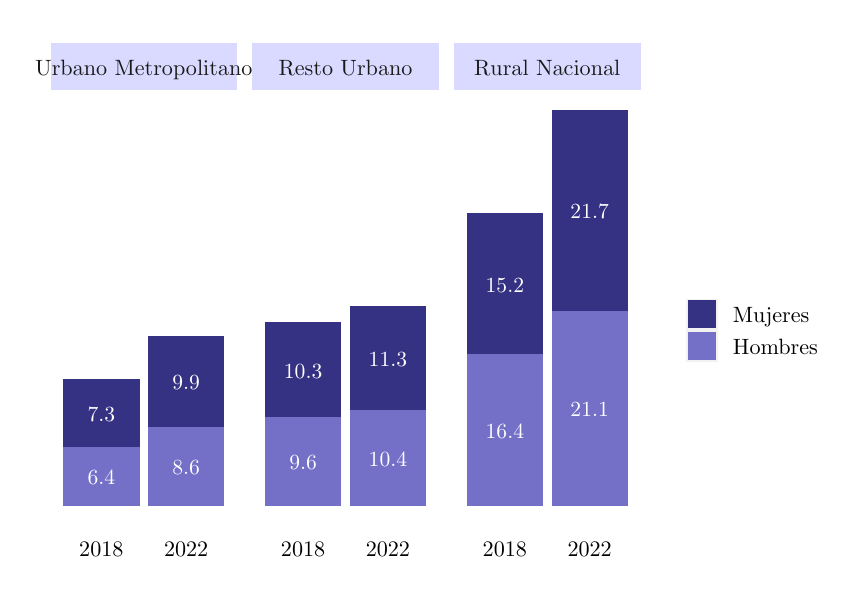
\begin{tikzpicture}[x=1pt,y=1pt]% Created by tikzDevice version 0.12.4 on 2023-05-10 12:06:09
% !TEX encoding = UTF-8 Unicode
\definecolor{fillColor}{RGB}{255,255,255}
\path[use as bounding box,fill=fillColor,fill opacity=0.00] (0,0) rectangle (289.08,198.74);
\begin{scope}
\path[clip] (  0.00,  0.00) rectangle (289.08,198.74);
\definecolor{drawColor}{RGB}{255,255,255}
\definecolor{fillColor}{RGB}{255,255,255}

\path[draw=drawColor,line width= 0.6pt,line join=round,line cap=round,fill=fillColor] (  0.00,  0.00) rectangle (289.08,198.74);
\end{scope}
\begin{scope}
\path[clip] (  0.00,  0.00) rectangle (289.08,198.74);
\definecolor{fillColor}{RGB}{54,50,131}

\path[fill=fillColor] ( 12.85, 47.35) rectangle ( 40.42, 71.61);
\definecolor{fillColor}{RGB}{116,112,200}

\path[fill=fillColor] ( 12.85, 25.96) rectangle ( 40.42, 47.35);
\definecolor{fillColor}{RGB}{54,50,131}

\path[fill=fillColor] ( 43.48, 54.56) rectangle ( 71.06, 87.47);
\definecolor{fillColor}{RGB}{116,112,200}

\path[fill=fillColor] ( 43.48, 25.96) rectangle ( 71.06, 54.56);
\definecolor{drawColor}{RGB}{255,255,255}

\node[text=drawColor,anchor=base,inner sep=0pt, outer sep=0pt, scale=  0.78] at ( 26.63, 56.45) {7.3};

\node[text=drawColor,anchor=base,inner sep=0pt, outer sep=0pt, scale=  0.78] at ( 26.63, 33.62) {6.4};

\node[text=drawColor,anchor=base,inner sep=0pt, outer sep=0pt, scale=  0.78] at ( 57.27, 67.98) {9.9};

\node[text=drawColor,anchor=base,inner sep=0pt, outer sep=0pt, scale=  0.78] at ( 57.27, 37.23) {8.6};
\end{scope}
\begin{scope}
\path[clip] (  0.00,  0.00) rectangle (289.08,198.74);
\definecolor{fillColor}{RGB}{54,50,131}

\path[fill=fillColor] ( 85.75, 58.03) rectangle (113.32, 92.32);
\definecolor{fillColor}{RGB}{116,112,200}

\path[fill=fillColor] ( 85.75, 25.96) rectangle (113.32, 58.03);
\definecolor{fillColor}{RGB}{54,50,131}

\path[fill=fillColor] (116.38, 60.51) rectangle (143.96, 98.34);
\definecolor{fillColor}{RGB}{116,112,200}

\path[fill=fillColor] (116.38, 25.96) rectangle (143.96, 60.51);
\definecolor{drawColor}{RGB}{255,255,255}

\node[text=drawColor,anchor=base,inner sep=0pt, outer sep=0pt, scale=  0.78] at ( 99.53, 72.14) {10.3};

\node[text=drawColor,anchor=base,inner sep=0pt, outer sep=0pt, scale=  0.78] at ( 99.53, 38.96) {9.6};

\node[text=drawColor,anchor=base,inner sep=0pt, outer sep=0pt, scale=  0.78] at (130.17, 76.39) {11.3};

\node[text=drawColor,anchor=base,inner sep=0pt, outer sep=0pt, scale=  0.78] at (130.17, 40.20) {10.4};
\end{scope}
\begin{scope}
\path[clip] (  0.00,  0.00) rectangle (289.08,198.74);
\definecolor{fillColor}{RGB}{54,50,131}

\path[fill=fillColor] (158.65, 80.79) rectangle (186.22,131.61);
\definecolor{fillColor}{RGB}{116,112,200}

\path[fill=fillColor] (158.65, 25.96) rectangle (186.22, 80.79);
\definecolor{fillColor}{RGB}{54,50,131}

\path[fill=fillColor] (189.29, 96.44) rectangle (216.86,168.94);
\definecolor{fillColor}{RGB}{116,112,200}

\path[fill=fillColor] (189.29, 25.96) rectangle (216.86, 96.44);
\definecolor{drawColor}{RGB}{255,255,255}

\node[text=drawColor,anchor=base,inner sep=0pt, outer sep=0pt, scale=  0.78] at (172.44,103.17) {15.2};

\node[text=drawColor,anchor=base,inner sep=0pt, outer sep=0pt, scale=  0.78] at (172.44, 50.34) {16.4};

\node[text=drawColor,anchor=base,inner sep=0pt, outer sep=0pt, scale=  0.78] at (203.07,129.65) {21.7};

\node[text=drawColor,anchor=base,inner sep=0pt, outer sep=0pt, scale=  0.78] at (203.07, 58.17) {21.1};
\end{scope}
\begin{scope}
\path[clip] (  0.00,  0.00) rectangle (289.08,198.74);
\definecolor{fillColor}{RGB}{218,217,255}

\path[fill=fillColor] (  8.25,176.08) rectangle ( 75.65,193.24);
\definecolor{drawColor}{gray}{0.10}

\node[text=drawColor,anchor=base,inner sep=0pt, outer sep=0pt, scale=  0.80] at ( 41.95,181.54) {Urbano Metropolitano};
\end{scope}
\begin{scope}
\path[clip] (  0.00,  0.00) rectangle (289.08,198.74);
\definecolor{fillColor}{RGB}{218,217,255}

\path[fill=fillColor] ( 81.15,176.08) rectangle (148.55,193.24);
\definecolor{drawColor}{gray}{0.10}

\node[text=drawColor,anchor=base,inner sep=0pt, outer sep=0pt, scale=  0.80] at (114.85,181.54) {Resto Urbano};
\end{scope}
\begin{scope}
\path[clip] (  0.00,  0.00) rectangle (289.08,198.74);
\definecolor{fillColor}{RGB}{218,217,255}

\path[fill=fillColor] (154.05,176.08) rectangle (221.46,193.24);
\definecolor{drawColor}{gray}{0.10}

\node[text=drawColor,anchor=base,inner sep=0pt, outer sep=0pt, scale=  0.80] at (187.75,181.54) {Rural Nacional};
\end{scope}
\begin{scope}
\path[clip] (  0.00,  0.00) rectangle (289.08,198.74);
\definecolor{drawColor}{RGB}{0,0,0}

\node[text=drawColor,anchor=base,inner sep=0pt, outer sep=0pt, scale=  0.80] at ( 26.63,  7.60) {2018};

\node[text=drawColor,anchor=base,inner sep=0pt, outer sep=0pt, scale=  0.80] at ( 57.27,  7.60) {2022};
\end{scope}
\begin{scope}
\path[clip] (  0.00,  0.00) rectangle (289.08,198.74);
\definecolor{drawColor}{RGB}{0,0,0}

\node[text=drawColor,anchor=base,inner sep=0pt, outer sep=0pt, scale=  0.80] at ( 99.53,  7.60) {2018};

\node[text=drawColor,anchor=base,inner sep=0pt, outer sep=0pt, scale=  0.80] at (130.17,  7.60) {2022};
\end{scope}
\begin{scope}
\path[clip] (  0.00,  0.00) rectangle (289.08,198.74);
\definecolor{drawColor}{RGB}{0,0,0}

\node[text=drawColor,anchor=base,inner sep=0pt, outer sep=0pt, scale=  0.80] at (172.44,  7.60) {2018};

\node[text=drawColor,anchor=base,inner sep=0pt, outer sep=0pt, scale=  0.80] at (203.07,  7.60) {2022};
\end{scope}
\begin{scope}
\path[clip] (  0.00,  0.00) rectangle (289.08,198.74);
\definecolor{fillColor}{RGB}{255,255,255}

\path[fill=fillColor] (232.46, 72.59) rectangle (283.58,122.30);
\end{scope}
\begin{scope}
\path[clip] (  0.00,  0.00) rectangle (289.08,198.74);
\definecolor{fillColor}{gray}{0.95}

\path[fill=fillColor] (237.96, 89.47) rectangle (249.34,100.85);
\end{scope}
\begin{scope}
\path[clip] (  0.00,  0.00) rectangle (289.08,198.74);
\definecolor{fillColor}{RGB}{54,50,131}

\path[fill=fillColor] (238.62, 90.14) rectangle (248.67,100.19);
\end{scope}
\begin{scope}
\path[clip] (  0.00,  0.00) rectangle (289.08,198.74);
\definecolor{fillColor}{gray}{0.95}

\path[fill=fillColor] (237.96, 78.09) rectangle (249.34, 89.47);
\end{scope}
\begin{scope}
\path[clip] (  0.00,  0.00) rectangle (289.08,198.74);
\definecolor{fillColor}{RGB}{116,112,200}

\path[fill=fillColor] (238.62, 78.75) rectangle (248.67, 88.81);
\end{scope}
\begin{scope}
\path[clip] (  0.00,  0.00) rectangle (289.08,198.74);
\definecolor{drawColor}{RGB}{0,0,0}

\node[text=drawColor,anchor=base west,inner sep=0pt, outer sep=0pt, scale=  0.80] at (254.84, 92.04) {Mujeres};
\end{scope}
\begin{scope}
\path[clip] (  0.00,  0.00) rectangle (289.08,198.74);
\definecolor{drawColor}{RGB}{0,0,0}

\node[text=drawColor,anchor=base west,inner sep=0pt, outer sep=0pt, scale=  0.80] at (254.84, 80.66) {Hombres};
\end{scope}
\end{tikzpicture}}{INE - ENEI 2022, ENEI 2 2018}{}

\cajita{Nivel educativo de la población de 15 años o más por sexo}{La tabla muestra la desagregación de la población de 15 años o más por sexo según el nivel educativo en el cual se reportó su último grado aprobado. 

En ambos años 2018 y 2022, se reportó un mayor porcentaje de mujeres que hombres sin ningún grado aprobado en ningún nivel educativo; en esta misma categoría, el porcentaje de mujeres incrementó de 2.5 puntos porcentuales de 2018 a 2022. 

Para 2022, el porcentaje de mujeres con algún grado aprobado en primaria o en diversificado fue mayor que los porcentajes de hombres respectivos. Similarmente, del 2018 al 2022 se reportó un aumento de dichas poblaciones de mujeres, 3.6 puntos porcentuales para primaria y 2.8 para diversificado. }{Nivel educativo de la población de 15 años o más por sexo (porcentaje)}{República de Guatemala, Instituto Nacional de Estadística}{\begin{tabular}[t]{ccccc}
\toprule
\multicolumn{1}{c}{\textbf{ }} & \multicolumn{2}{c}{\textbf{2018}} & \multicolumn{2}{c}{\textbf{2022}} \\
\cmidrule(l{3pt}r{3pt}){2-3} \cmidrule(l{3pt}r{3pt}){4-5}
\textbf{Nivel Educativo} & \textbf{Mujeres} & \textbf{Hombres} & \textbf{Mujeres} & \textbf{Hombres}\\
\midrule
\cellcolor[HTML]{B6B3FF}{Ninguno} & \cellcolor[HTML]{B6B3FF}{9.9} & \cellcolor[HTML]{B6B3FF}{5.0} & \cellcolor[HTML]{B6B3FF}{12.4} & \cellcolor[HTML]{B6B3FF}{6.2}\\
Preprimaria & 0.1 & 0.1 & 0.9 & 0.7\\
\cellcolor[HTML]{B6B3FF}{Primaria} & \cellcolor[HTML]{B6B3FF}{16.2} & \cellcolor[HTML]{B6B3FF}{15.5} & \cellcolor[HTML]{B6B3FF}{19.8} & \cellcolor[HTML]{B6B3FF}{17.0}\\
Básico & 6.0 & 6.4 & 7.7 & 8.5\\
\cellcolor[HTML]{B6B3FF}{Diversificado} & \cellcolor[HTML]{B6B3FF}{7.6} & \cellcolor[HTML]{B6B3FF}{7.6} & \cellcolor[HTML]{B6B3FF}{10.4} & \cellcolor[HTML]{B6B3FF}{9.3}\\
Superior & 2.2 & 2.2 & 3.2 & 3.4\\
\cellcolor[HTML]{B6B3FF}{Posgrado} & \cellcolor[HTML]{B6B3FF}{0.1} & \cellcolor[HTML]{B6B3FF}{0.1} & \cellcolor[HTML]{B6B3FF}{0.3} & \cellcolor[HTML]{B6B3FF}{0.3}\\
\bottomrule
\end{tabular}
}{INE - ENEI 2022, ENEI 2 2018}{}

\cajita{REVISAR Tasa neta de escolaridad en el nivel primario por sexo}{La tasa neta de escolaridad es la relaciónporcentual entre el alumnado de la edad tradicional de completación del nivel educativo sobre el total de la población de esa edad.

La gráfica muestra que en Guatemala, la tasa neta de escolaridad en el nivel primario de mujeres sobrepasó la de los hombres en 2020 y 2022. Entre 2018 y 2022, la tasa aumentó en
2.5 puntos porcentuales para las mujeres.}{Tasa neta de escolaridad en el nivel primario por sexo (porcentaje)}{República de Guatemala, Instituto Nacional de Estadística}{\begin{tikzpicture}[x=1pt,y=1pt]% Created by tikzDevice version 0.12.4 on 2023-05-31 15:10:30
% !TEX encoding = UTF-8 Unicode
\definecolor{fillColor}{RGB}{255,255,255}
\path[use as bounding box,fill=fillColor,fill opacity=0.00] (0,0) rectangle (289.08,198.74);
\begin{scope}
\path[clip] (  0.00,  0.00) rectangle (289.08,198.74);

\path[] (  0.00,  0.00) rectangle (289.08,198.74);
\end{scope}
\begin{scope}
\path[clip] (  0.00,  0.00) rectangle (289.08,198.74);
\definecolor{drawColor}{RGB}{54,50,131}

\path[draw=drawColor,line width= 1.7pt,line join=round] ( 35.79, 82.38) --
	( 88.99,124.94) --
	(142.20,113.88) --
	(195.41,108.90) --
	(248.62,103.39);
\definecolor{drawColor}{RGB}{116,112,200}

\path[draw=drawColor,line width= 1.7pt,line join=round] ( 35.79, 82.41) --
	( 88.99,124.63) --
	(142.20,110.19) --
	(195.41,100.01) --
	(248.62, 95.74);
\definecolor{drawColor}{RGB}{0,0,0}

\node[text=drawColor,anchor=base,inner sep=0pt, outer sep=0pt, scale=  1.02] at ( 35.79, 70.47) { };

\node[text=drawColor,anchor=base,inner sep=0pt, outer sep=0pt, scale=  1.02] at ( 88.99,128.91) { };

\node[text=drawColor,anchor=base west,inner sep=0pt, outer sep=0pt, scale=  1.02] at (142.20,120.85) {93.9};

\node[text=drawColor,anchor=base west,inner sep=0pt, outer sep=0pt, scale=  1.02] at (195.41,112.87) {93.3};

\node[text=drawColor,anchor=base,inner sep=0pt, outer sep=0pt, scale=  1.02] at (248.62, 108.47) {92.7};

\node[text=drawColor,anchor=base,inner sep=0pt, outer sep=0pt, scale=  1.02] at ( 35.79, 67.50) {90.2};

\node[text=drawColor,anchor=base,inner sep=0pt, outer sep=0pt, scale=  1.02] at ( 88.99,128.60) {95.2};

\node[text=drawColor,anchor=base west,inner sep=0pt, outer sep=0pt, scale=  1.02] at (142.20,94.16) {93.5};

\node[text=drawColor,anchor=base west,inner sep=0pt, outer sep=0pt, scale=  1.02] at (195.41,84.98) {92.3};

\node[text=drawColor,anchor=base,inner sep=0pt, outer sep=0pt, scale=  1.02] at (248.62, 80.83) {91.8};

\path[draw=drawColor,line width= 0.1pt,line join=round] (-272.82, 23.41) -- (557.23, 23.41);

\path[] (  3.86, 15.40) rectangle (280.54,191.63);

\path[] (  3.86, 17.51) --
	(280.54, 17.51);

\path[] (  3.86, 59.67) --
	(280.54, 59.67);

\path[] (  3.86,101.83) --
	(280.54,101.83);

\path[] (  3.86,143.99) --
	(280.54,143.99);

\path[] (  3.86,186.15) --
	(280.54,186.15);

\path[] (  3.86, 38.59) --
	(280.54, 38.59);

\path[] (  3.86, 80.75) --
	(280.54, 80.75);

\path[] (  3.86,122.91) --
	(280.54,122.91);

\path[] (  3.86,165.07) --
	(280.54,165.07);

\path[] ( 35.79, 15.40) --
	( 35.79,191.63);

\path[] ( 88.99, 15.40) --
	( 88.99,191.63);

\path[] (142.20, 15.40) --
	(142.20,191.63);

\path[] (195.41, 15.40) --
	(195.41,191.63);

\path[] (248.62, 15.40) --
	(248.62,191.63);

\path[] (  3.86, 15.40) rectangle (280.54,191.63);
\end{scope}
\begin{scope}
\path[clip] (  0.00,  0.00) rectangle (289.08,198.74);

\path[] (  3.86, 15.40) --
	(  3.86,191.63);
\end{scope}
\begin{scope}
\path[clip] (  0.00,  0.00) rectangle (289.08,198.74);
\definecolor{drawColor}{RGB}{255,255,255}

\node[text=drawColor,text opacity=0.00,anchor=base east,inner sep=0pt, outer sep=0pt, scale=  1.00] at ( -1.09, 34.68) {85};

\node[text=drawColor,text opacity=0.00,anchor=base east,inner sep=0pt, outer sep=0pt, scale=  1.00] at ( -1.09, 76.84) {90};

\node[text=drawColor,text opacity=0.00,anchor=base east,inner sep=0pt, outer sep=0pt, scale=  1.00] at ( -1.09,119.00) {95};

\node[text=drawColor,text opacity=0.00,anchor=base east,inner sep=0pt, outer sep=0pt, scale=  1.00] at ( -1.09,161.16) {100};
\end{scope}
\begin{scope}
\path[clip] (  0.00,  0.00) rectangle (289.08,198.74);

\path[] (  1.11, 38.59) --
	(  3.86, 38.59);

\path[] (  1.11, 80.75) --
	(  3.86, 80.75);

\path[] (  1.11,122.91) --
	(  3.86,122.91);

\path[] (  1.11,165.07) --
	(  3.86,165.07);
\end{scope}
\begin{scope}
\path[clip] (  0.00,  0.00) rectangle (289.08,198.74);

\path[] (  3.86, 15.40) --
	(280.54, 15.40);
\end{scope}
\begin{scope}
\path[clip] (  0.00,  0.00) rectangle (289.08,198.74);

\path[] ( 35.79, 12.65) --
	( 35.79, 15.40);

\path[] ( 88.99, 12.65) --
	( 88.99, 15.40);

\path[] (142.20, 12.65) --
	(142.20, 15.40);

\path[] (195.41, 12.65) --
	(195.41, 15.40);

\path[] (248.62, 12.65) --
	(248.62, 15.40);
\end{scope}
\begin{scope}
\path[clip] (  0.00,  0.00) rectangle (289.08,198.74);
\definecolor{drawColor}{RGB}{0,0,0}

\node[text=drawColor,anchor=base,inner sep=0pt, outer sep=0pt, scale=  1.00] at ( 35.79,  1.32) {2018};

\node[text=drawColor,anchor=base,inner sep=0pt, outer sep=0pt, scale=  1.00] at ( 88.99,  1.32) {2019};

\node[text=drawColor,anchor=base,inner sep=0pt, outer sep=0pt, scale=  1.00] at (142.20,  1.32) {2020};

\node[text=drawColor,anchor=base,inner sep=0pt, outer sep=0pt, scale=  1.00] at (195.41,  1.32) {2021};

\node[text=drawColor,anchor=base,inner sep=0pt, outer sep=0pt, scale=  1.00] at (248.62,  1.32) {2022};
\end{scope}
\begin{scope}
\path[clip] (  0.00,  0.00) rectangle (289.08,198.74);
\coordinate (apoyo) at (58.34,189.21);
\coordinate (longitudFicticia) at (7.11,9.53);
\coordinate (longitud) at (7.11,7.11);
\coordinate (desX) at (134.96,0);
\coordinate (desY) at (0,1.21);
\definecolor[named]{ct1}{HTML}{
363283
}
\definecolor[named]{ct2}{HTML}{
7470C8
}
\definecolor[named]{ctb1}{HTML}{
363283
}
\definecolor[named]{ctb2}{HTML}{
7470C8
}
\path [fill=none] (apoyo) rectangle ($(apoyo)+(longitudFicticia)$)
node [xshift=0.3cm,inner sep=0pt, outer sep=0pt,midway,right,scale = 1]{Mujeres};
\draw [color = ctb1,fill=ct1] ( $(apoyo)  + (desY) $) rectangle ($(apoyo)+ (desY) +(longitud)$);
\path [fill=none] ($(apoyo)+(desX)$) rectangle ($(apoyo)+(desX)+(longitudFicticia)$)
node [xshift=0.3cm,inner sep=0pt, outer sep=0pt,midway,right,scale = 1]{Hombres};
\draw [color = ctb2 ,fill=ct2] ( $(apoyo)  + (desY) + (desX) $) rectangle ($(apoyo)+ (desY)+ (desX) +(longitud)$);
\end{scope}
\end{tikzpicture}}{Estadísticas de Educación INE, con datos proporcionados por el Ministerio de Educación}{}

\cajota{REVISAR Tasa neta de escolaridad en el nivel primario por sexo, según departamento}{La tabla muestra que en Guatemala, la tasa neta de escolaridad en el nivel primario de mujeres más baja reportada entre 2018 y 2022 fue en Suchitepéquez con 79.5. Dicha tasa aumentó a 93.1 para 2022.

De 2018 a 2022 las tasas netas de escolaridad en el nivel primario de mujeres en Guatemala sobrepasaron la de hombres. }{Tasa neta de escolaridad en el nivel primario por sexo, según departamento (porcentaje)}{República de Guatemala, Instituto Nacional de Estadística}{\centering\resizebox{\textwidth}{!}{\begin{tabular}[t]{ccccccccc}
\toprule
\multicolumn{1}{c}{\textbf{ }} & \multicolumn{2}{c}{\textbf{2018}} & \multicolumn{2}{c}{\textbf{2019}} & \multicolumn{2}{c}{\textbf{2020}} & \multicolumn{2}{c}{\textbf{2021}} \\
\cmidrule(l{3pt}r{3pt}){2-3} \cmidrule(l{3pt}r{3pt}){4-5} \cmidrule(l{3pt}r{3pt}){6-7} \cmidrule(l{3pt}r{3pt}){8-9}
\textbf{Departamento} & \textbf{Mujeres} & \textbf{Hombres} & \textbf{Mujeres} & \textbf{Hombres} & \textbf{Mujeres} & \textbf{Hombres} & \textbf{Mujeres} & \textbf{Hombres}\\
\midrule
\cellcolor[HTML]{B6B3FF}{Guatemala} & \cellcolor[HTML]{B6B3FF}{100.1} & \cellcolor[HTML]{B6B3FF}{99.2} & \cellcolor[HTML]{B6B3FF}{106.4} & \cellcolor[HTML]{B6B3FF}{105.6} & \cellcolor[HTML]{B6B3FF}{104.0} & \cellcolor[HTML]{B6B3FF}{103.0} & \cellcolor[HTML]{B6B3FF}{100.8} & \cellcolor[HTML]{B6B3FF}{99.5}\\
El Progreso & 92.7 & 94.8 & 100.8 & 105.2 & 97.7 & 102.4 & 98.6 & 103.5\\
\cellcolor[HTML]{B6B3FF}{Sacatepéquez} & \cellcolor[HTML]{B6B3FF}{94.8} & \cellcolor[HTML]{B6B3FF}{93.9} & \cellcolor[HTML]{B6B3FF}{99.6} & \cellcolor[HTML]{B6B3FF}{99.3} & \cellcolor[HTML]{B6B3FF}{98.7} & \cellcolor[HTML]{B6B3FF}{98.4} & \cellcolor[HTML]{B6B3FF}{97.2} & \cellcolor[HTML]{B6B3FF}{96.5}\\
Chimaltenango & 90.0 & 87.9 & 92.4 & 91.1 & 92.3 & 90.7 & 94.5 & 92.8\\
\cellcolor[HTML]{B6B3FF}{Escuintla} & \cellcolor[HTML]{B6B3FF}{90.9} & \cellcolor[HTML]{B6B3FF}{94.1} & \cellcolor[HTML]{B6B3FF}{102.4} & \cellcolor[HTML]{B6B3FF}{105.5} & \cellcolor[HTML]{B6B3FF}{99.7} & \cellcolor[HTML]{B6B3FF}{102.4} & \cellcolor[HTML]{B6B3FF}{98.7} & \cellcolor[HTML]{B6B3FF}{100.7}\\
Santa Rosa & 91.0 & 91.9 & 99.4 & 99.6 & 97.3 & 96.3 & 95.6 & 94.4\\
\cellcolor[HTML]{B6B3FF}{Sololá} & \cellcolor[HTML]{B6B3FF}{88.7} & \cellcolor[HTML]{B6B3FF}{88.9} & \cellcolor[HTML]{B6B3FF}{94.0} & \cellcolor[HTML]{B6B3FF}{93.6} & \cellcolor[HTML]{B6B3FF}{94.4} & \cellcolor[HTML]{B6B3FF}{94.1} & \cellcolor[HTML]{B6B3FF}{96.0} & \cellcolor[HTML]{B6B3FF}{94.5}\\
Totonicapán & 85.5 & 83.3 & 87.5 & 84.9 & 86.6 & 84.0 & 85.7 & 83.3\\
\cellcolor[HTML]{B6B3FF}{Quetzaltenango} & \cellcolor[HTML]{B6B3FF}{90.6} & \cellcolor[HTML]{B6B3FF}{92.3} & \cellcolor[HTML]{B6B3FF}{96.6} & \cellcolor[HTML]{B6B3FF}{97.8} & \cellcolor[HTML]{B6B3FF}{95.9} & \cellcolor[HTML]{B6B3FF}{96.5} & \cellcolor[HTML]{B6B3FF}{94.2} & \cellcolor[HTML]{B6B3FF}{94.0}\\
Suchitepéquez & 79.5 & 81.2 & 87.0 & 88.5 & 88.6 & 90.0 & 92.5 & 92.4\\
\cellcolor[HTML]{B6B3FF}{Retalhuleu} & \cellcolor[HTML]{B6B3FF}{88.3} & \cellcolor[HTML]{B6B3FF}{86.5} & \cellcolor[HTML]{B6B3FF}{95.1} & \cellcolor[HTML]{B6B3FF}{94.4} & \cellcolor[HTML]{B6B3FF}{93.8} & \cellcolor[HTML]{B6B3FF}{91.6} & \cellcolor[HTML]{B6B3FF}{93.7} & \cellcolor[HTML]{B6B3FF}{91.3}\\
San Marcos & 87.6 & 87.8 & 91.8 & 92.2 & 91.2 & 91.4 & 91.3 & 90.7\\
\cellcolor[HTML]{B6B3FF}{Huehuetenango} & \cellcolor[HTML]{B6B3FF}{86.8} & \cellcolor[HTML]{B6B3FF}{85.7} & \cellcolor[HTML]{B6B3FF}{88.1} & \cellcolor[HTML]{B6B3FF}{86.3} & \cellcolor[HTML]{B6B3FF}{87.2} & \cellcolor[HTML]{B6B3FF}{84.5} & \cellcolor[HTML]{B6B3FF}{86.5} & \cellcolor[HTML]{B6B3FF}{83.1}\\
Quiché & 88.3 & 88.2 & 90.0 & 89.9 & 88.6 & 88.5 & 88.6 & 88.1\\
\cellcolor[HTML]{B6B3FF}{Baja Verapaz} & \cellcolor[HTML]{B6B3FF}{84.8} & \cellcolor[HTML]{B6B3FF}{85.4} & \cellcolor[HTML]{B6B3FF}{89.0} & \cellcolor[HTML]{B6B3FF}{89.7} & \cellcolor[HTML]{B6B3FF}{85.6} & \cellcolor[HTML]{B6B3FF}{86.6} & \cellcolor[HTML]{B6B3FF}{85.6} & \cellcolor[HTML]{B6B3FF}{86.2}\\
Alta Verapaz & 88.1 & 88.1 & 91.3 & 91.6 & 90.5 & 90.7 & 91.3 & 90.6\\
\cellcolor[HTML]{B6B3FF}{Petén} & \cellcolor[HTML]{B6B3FF}{89.8} & \cellcolor[HTML]{B6B3FF}{89.7} & \cellcolor[HTML]{B6B3FF}{99.5} & \cellcolor[HTML]{B6B3FF}{99.1} & \cellcolor[HTML]{B6B3FF}{95.7} & \cellcolor[HTML]{B6B3FF}{95.2} & \cellcolor[HTML]{B6B3FF}{93.0} & \cellcolor[HTML]{B6B3FF}{91.6}\\
Izabal & 91.7 & 92.3 & 99.3 & 99.9 & 97.6 & 97.6 & 96.9 & 96.0\\
\cellcolor[HTML]{B6B3FF}{Zacapa} & \cellcolor[HTML]{B6B3FF}{86.8} & \cellcolor[HTML]{B6B3FF}{90.0} & \cellcolor[HTML]{B6B3FF}{92.7} & \cellcolor[HTML]{B6B3FF}{96.6} & \cellcolor[HTML]{B6B3FF}{91.6} & \cellcolor[HTML]{B6B3FF}{94.0} & \cellcolor[HTML]{B6B3FF}{91.2} & \cellcolor[HTML]{B6B3FF}{93.3}\\
Chiquimula & 87.9 & 89.6 & 92.7 & 93.3 & 91.7 & 91.5 & 91.1 & 90.8\\
\cellcolor[HTML]{B6B3FF}{Jalapa} & \cellcolor[HTML]{B6B3FF}{84.8} & \cellcolor[HTML]{B6B3FF}{85.3} & \cellcolor[HTML]{B6B3FF}{89.5} & \cellcolor[HTML]{B6B3FF}{89.7} & \cellcolor[HTML]{B6B3FF}{88.5} & \cellcolor[HTML]{B6B3FF}{88.7} & \cellcolor[HTML]{B6B3FF}{89.8} & \cellcolor[HTML]{B6B3FF}{88.7}\\
Jutiapa & 89.4 & 89.1 & 95.9 & 95.7 & 94.8 & 92.7 & 94.9 & 91.6\\
\bottomrule
\end{tabular}}
}{Estadísticas de Educación INE, con datos proporcionados por el Ministerio de Educación}

\cajita{REVISAR Tasa neta de escolaridad en el ciclo básico por sexo}{La tasa neta de escolaridad es la relaciónporcentual entre el alumnado de la edad tradicional de completación del nivel educativo sobre el total de la población de esa edad.

La gráfica muestra que en Guatemala, la tasa neta de escolaridad en el nivel primario de mujeres sobrepasó la de los hombres en 2020 y 2022. Entre 2018 y 2022, la tasa aumentó en
2.5 puntos porcentuales para las mujeres.}{Tasa neta de escolaridad en el ciclo básico por sexo (porcentaje)}{República de Guatemala, Instituto Nacional de Estadística}{\begin{tikzpicture}[x=1pt,y=1pt]% Created by tikzDevice version 0.12.4 on 2023-05-31 15:27:59
% !TEX encoding = UTF-8 Unicode
\definecolor{fillColor}{RGB}{255,255,255}
\path[use as bounding box,fill=fillColor,fill opacity=0.00] (0,0) rectangle (289.08,198.74);
\begin{scope}
\path[clip] (  0.00,  0.00) rectangle (289.08,198.74);

\path[] (  0.00,  0.00) rectangle (289.08,198.74);
\end{scope}
\begin{scope}
\path[clip] (  0.00,  0.00) rectangle (289.08,198.74);
\definecolor{drawColor}{RGB}{54,50,131}

\path[draw=drawColor,line width= 1.7pt,line join=round] ( 31.91,107.16) --
	( 85.96,117.25) --
	(140.01,114.29) --
	(194.06, 95.52) --
	(248.11,107.92);
\definecolor{drawColor}{RGB}{116,112,200}

\path[draw=drawColor,line width= 1.7pt,line join=round] ( 31.91,114.92) --
	( 85.96,121.26) --
	(140.01,118.27) --
	(194.06, 86.00) --
	(248.11, 99.35);
\definecolor{drawColor}{RGB}{0,0,0}

\node[text=drawColor,anchor=base,inner sep=0pt, outer sep=0pt, scale=  1.02] at ( 31.91, 92.25) {47.6};

\node[text=drawColor,anchor=base,inner sep=0pt, outer sep=0pt, scale=  1.02] at ( 85.96,102.22) {49.4};

\node[text=drawColor,anchor=base west,inner sep=0pt, outer sep=0pt, scale=  1.02] at (140.01,98.26) {48.9};

\node[text=drawColor,anchor=base,inner sep=0pt, outer sep=0pt, scale=  1.02] at (194.06, 103.61) {45.5};

\node[text=drawColor,anchor=base,inner sep=0pt, outer sep=0pt, scale=  1.02] at (248.11,111.89) {47.7};

\node[text=drawColor,anchor=base,inner sep=0pt, outer sep=0pt, scale=  1.02] at ( 31.91,118.01) {49.0};

\node[text=drawColor,anchor=base,inner sep=0pt, outer sep=0pt, scale=  1.02] at ( 85.96,125.23) {50.1};

\node[text=drawColor,anchor=base west,inner sep=0pt, outer sep=0pt, scale=  1.02] at (140.01,122.24) {49.6};

\node[text=drawColor,anchor=base,inner sep=0pt, outer sep=0pt, scale=  1.02] at (194.06, 74.08) {43.9};

\node[text=drawColor,anchor=base,inner sep=0pt, outer sep=0pt, scale=  1.02] at (248.11,87.32) {46.2};

\path[draw=drawColor,line width= 0.1pt,line join=round] (-281.58, 23.41) -- (561.61, 23.41);

\path[] ( -0.52, 15.40) rectangle (280.54,191.63);

\path[] ( -0.52, 35.86) --
	(280.54, 35.86);

\path[] ( -0.52, 92.47) --
	(280.54, 92.47);

\path[] ( -0.52,149.09) --
	(280.54,149.09);

\path[] ( -0.52, 64.17) --
	(280.54, 64.17);

\path[] ( -0.52,120.78) --
	(280.54,120.78);

\path[] ( -0.52,177.39) --
	(280.54,177.39);

\path[] ( 31.91, 15.40) --
	( 31.91,191.63);

\path[] ( 85.96, 15.40) --
	( 85.96,191.63);

\path[] (140.01, 15.40) --
	(140.01,191.63);

\path[] (194.06, 15.40) --
	(194.06,191.63);

\path[] (248.11, 15.40) --
	(248.11,191.63);

\path[] ( -0.52, 15.40) rectangle (280.54,191.63);
\end{scope}
\begin{scope}
\path[clip] (  0.00,  0.00) rectangle (289.08,198.74);

\path[] ( -0.52, 15.40) --
	( -0.52,191.63);
\end{scope}
\begin{scope}
\path[clip] (  0.00,  0.00) rectangle (289.08,198.74);
\definecolor{drawColor}{RGB}{255,255,255}

\node[text=drawColor,text opacity=0.00,anchor=base east,inner sep=0pt, outer sep=0pt, scale=  1.00] at ( -5.47, 60.26) {40};

\node[text=drawColor,text opacity=0.00,anchor=base east,inner sep=0pt, outer sep=0pt, scale=  1.00] at ( -5.47,116.87) {50};

\node[text=drawColor,text opacity=0.00,anchor=base east,inner sep=0pt, outer sep=0pt, scale=  1.00] at ( -5.47,173.48) {60};
\end{scope}
\begin{scope}
\path[clip] (  0.00,  0.00) rectangle (289.08,198.74);

\path[] ( -3.27, 64.17) --
	( -0.52, 64.17);

\path[] ( -3.27,120.78) --
	( -0.52,120.78);

\path[] ( -3.27,177.39) --
	( -0.52,177.39);
\end{scope}
\begin{scope}
\path[clip] (  0.00,  0.00) rectangle (289.08,198.74);

\path[] ( -0.52, 15.40) --
	(280.54, 15.40);
\end{scope}
\begin{scope}
\path[clip] (  0.00,  0.00) rectangle (289.08,198.74);

\path[] ( 31.91, 12.65) --
	( 31.91, 15.40);

\path[] ( 85.96, 12.65) --
	( 85.96, 15.40);

\path[] (140.01, 12.65) --
	(140.01, 15.40);

\path[] (194.06, 12.65) --
	(194.06, 15.40);

\path[] (248.11, 12.65) --
	(248.11, 15.40);
\end{scope}
\begin{scope}
\path[clip] (  0.00,  0.00) rectangle (289.08,198.74);
\definecolor{drawColor}{RGB}{0,0,0}

\node[text=drawColor,anchor=base,inner sep=0pt, outer sep=0pt, scale=  1.00] at ( 31.91,  1.32) {2018};

\node[text=drawColor,anchor=base,inner sep=0pt, outer sep=0pt, scale=  1.00] at ( 85.96,  1.32) {2019};

\node[text=drawColor,anchor=base,inner sep=0pt, outer sep=0pt, scale=  1.00] at (140.01,  1.32) {2020};

\node[text=drawColor,anchor=base,inner sep=0pt, outer sep=0pt, scale=  1.00] at (194.06,  1.32) {2021};

\node[text=drawColor,anchor=base,inner sep=0pt, outer sep=0pt, scale=  1.00] at (248.11,  1.32) {2022};
\end{scope}
\begin{scope}
\path[clip] (  0.00,  0.00) rectangle (289.08,198.74);
\coordinate (apoyo) at (58.34,189.21);
\coordinate (longitudFicticia) at (7.11,9.53);
\coordinate (longitud) at (7.11,7.11);
\coordinate (desX) at (134.96,0);
\coordinate (desY) at (0,1.21);
\definecolor[named]{ct1}{HTML}{
363283
}
\definecolor[named]{ct2}{HTML}{
7470C8
}
\definecolor[named]{ctb1}{HTML}{
363283
}
\definecolor[named]{ctb2}{HTML}{
7470C8
}
\path [fill=none] (apoyo) rectangle ($(apoyo)+(longitudFicticia)$)
node [xshift=0.3cm,inner sep=0pt, outer sep=0pt,midway,right,scale = 1]{Mujer};
\draw [color = ctb1,fill=ct1] ( $(apoyo)  + (desY) $) rectangle ($(apoyo)+ (desY) +(longitud)$);
\path [fill=none] ($(apoyo)+(desX)$) rectangle ($(apoyo)+(desX)+(longitudFicticia)$)
node [xshift=0.3cm,inner sep=0pt, outer sep=0pt,midway,right,scale = 1]{Hombre};
\draw [color = ctb2 ,fill=ct2] ( $(apoyo)  + (desY) + (desX) $) rectangle ($(apoyo)+ (desY)+ (desX) +(longitud)$);
\end{scope}
\end{tikzpicture}}{Estadísticas de Educación INE, con datos proporcionados por el Ministerio de Educación}{}

\cajita{REVISAR Tasa neta de escolaridad en el ciclo diversificado por sexo}{La gráfica muestra que, en Guatemala, la tasa neta de escolaridad en el ciclo diversificado
de las mujeres sobrepasó la de los hombres de 2018 a 2022. Para 2018 se reportó una tasa neta de mujeres de 26.5 y 25.6 en 2022.}{Tasa neta de escolaridad en el ciclo diversificado por sexo (porcentaje)}{República de Guatemala, Instituto Nacional de Estadística}{\begin{tikzpicture}[x=1pt,y=1pt]% Created by tikzDevice version 0.12.4 on 2023-05-29 13:32:28
% !TEX encoding = UTF-8 Unicode
\definecolor{fillColor}{RGB}{255,255,255}
\path[use as bounding box,fill=fillColor,fill opacity=0.00] (0,0) rectangle (289.08,198.74);
\begin{scope}
\path[clip] (  0.00,  0.00) rectangle (289.08,198.74);

\path[] (  0.00,  0.00) rectangle (289.08,198.74);
\end{scope}
\begin{scope}
\path[clip] (  0.00,  0.00) rectangle (289.08,198.74);
\definecolor{drawColor}{RGB}{54,50,131}

\path[draw=drawColor,line width= 1.7pt,line join=round] ( 39.63,159.54) --
	(106.55,176.61) --
	(173.47,182.05) --
	(240.39,139.83);
\definecolor{drawColor}{RGB}{116,112,200}

\path[draw=drawColor,line width= 1.7pt,line join=round] ( 39.63,108.10) --
	(106.55,122.27) --
	(173.47,124.67) --
	(240.39, 47.91);
\definecolor{drawColor}{RGB}{0,0,0}

\node[text=drawColor,anchor=base,inner sep=0pt, outer sep=0pt, scale=  1.02] at ( 39.63,147.63) {26.4};

\node[text=drawColor,anchor=base east,inner sep=0pt, outer sep=0pt, scale=  1.02] at (103.43,178.61) {27.2};

\node[text=drawColor,anchor=base,inner sep=0pt, outer sep=0pt, scale=  1.02] at (173.47,186.02) {27.4};

\node[text=drawColor,anchor=base,inner sep=0pt, outer sep=0pt, scale=  1.02] at (240.39,127.91) {25.6};

\node[text=drawColor,anchor=base,inner sep=0pt, outer sep=0pt, scale=  1.02] at ( 39.63, 96.18) {24.2};

\node[text=drawColor,anchor=base east,inner sep=0pt, outer sep=0pt, scale=  1.02] at (103.43,124.27) {24.8};

\node[text=drawColor,anchor=base,inner sep=0pt, outer sep=0pt, scale=  1.02] at (173.47,128.64) {24.9};

\node[text=drawColor,anchor=base,inner sep=0pt, outer sep=0pt, scale=  1.02] at (240.39, 36.00) {21.6};

\path[draw=drawColor,line width= 0.1pt,line join=round] (-281.58, 23.41) -- (561.61, 23.41);

\path[] ( -0.52, 15.40) rectangle (280.54,191.63);

\path[] ( -0.52, 34.85) --
	(280.54, 34.85);

\path[] ( -0.52, 80.63) --
	(280.54, 80.63);

\path[] ( -0.52,126.40) --
	(280.54,126.40);

\path[] ( -0.52,172.18) --
	(280.54,172.18);

\path[] ( -0.52, 57.74) --
	(280.54, 57.74);

\path[] ( -0.52,103.51) --
	(280.54,103.51);

\path[] ( -0.52,149.29) --
	(280.54,149.29);

\path[] ( 39.63, 15.40) --
	( 39.63,191.63);

\path[] (106.55, 15.40) --
	(106.55,191.63);

\path[] (173.47, 15.40) --
	(173.47,191.63);

\path[] (240.39, 15.40) --
	(240.39,191.63);

\path[] ( -0.52, 15.40) rectangle (280.54,191.63);
\end{scope}
\begin{scope}
\path[clip] (  0.00,  0.00) rectangle (289.08,198.74);

\path[] ( -0.52, 15.40) --
	( -0.52,191.63);
\end{scope}
\begin{scope}
\path[clip] (  0.00,  0.00) rectangle (289.08,198.74);
\definecolor{drawColor}{RGB}{255,255,255}

\node[text=drawColor,text opacity=0.00,anchor=base east,inner sep=0pt, outer sep=0pt, scale=  1.00] at ( -5.47, 53.83) {22};

\node[text=drawColor,text opacity=0.00,anchor=base east,inner sep=0pt, outer sep=0pt, scale=  1.00] at ( -5.47, 99.60) {24};

\node[text=drawColor,text opacity=0.00,anchor=base east,inner sep=0pt, outer sep=0pt, scale=  1.00] at ( -5.47,145.38) {26};
\end{scope}
\begin{scope}
\path[clip] (  0.00,  0.00) rectangle (289.08,198.74);

\path[] ( -3.27, 57.74) --
	( -0.52, 57.74);

\path[] ( -3.27,103.51) --
	( -0.52,103.51);

\path[] ( -3.27,149.29) --
	( -0.52,149.29);
\end{scope}
\begin{scope}
\path[clip] (  0.00,  0.00) rectangle (289.08,198.74);

\path[] ( -0.52, 15.40) --
	(280.54, 15.40);
\end{scope}
\begin{scope}
\path[clip] (  0.00,  0.00) rectangle (289.08,198.74);

\path[] ( 39.63, 12.65) --
	( 39.63, 15.40);

\path[] (106.55, 12.65) --
	(106.55, 15.40);

\path[] (173.47, 12.65) --
	(173.47, 15.40);

\path[] (240.39, 12.65) --
	(240.39, 15.40);
\end{scope}
\begin{scope}
\path[clip] (  0.00,  0.00) rectangle (289.08,198.74);
\definecolor{drawColor}{RGB}{0,0,0}

\node[text=drawColor,anchor=base,inner sep=0pt, outer sep=0pt, scale=  1.00] at ( 39.63,  1.32) {2018};

\node[text=drawColor,anchor=base,inner sep=0pt, outer sep=0pt, scale=  1.00] at (106.55,  1.32) {2019};

\node[text=drawColor,anchor=base,inner sep=0pt, outer sep=0pt, scale=  1.00] at (173.47,  1.32) {2020};

\node[text=drawColor,anchor=base,inner sep=0pt, outer sep=0pt, scale=  1.00] at (240.39,  1.32) {2021};
\end{scope}
\begin{scope}
\path[clip] (  0.00,  0.00) rectangle (289.08,198.74);
\coordinate (apoyo) at (58.34,189.21);
\coordinate (longitudFicticia) at (7.11,9.53);
\coordinate (longitud) at (7.11,7.11);
\coordinate (desX) at (134.96,0);
\coordinate (desY) at (0,1.21);
\definecolor[named]{ct1}{HTML}{
363283
}
\definecolor[named]{ct2}{HTML}{
7470C8
}
\definecolor[named]{ctb1}{HTML}{
363283
}
\definecolor[named]{ctb2}{HTML}{
7470C8
}
\path [fill=none] (apoyo) rectangle ($(apoyo)+(longitudFicticia)$)
node [xshift=0.3cm,inner sep=0pt, outer sep=0pt,midway,right,scale = 1]{Mujer};
\draw [color = ctb1,fill=ct1] ( $(apoyo)  + (desY) $) rectangle ($(apoyo)+ (desY) +(longitud)$);
\path [fill=none] ($(apoyo)+(desX)$) rectangle ($(apoyo)+(desX)+(longitudFicticia)$)
node [xshift=0.3cm,inner sep=0pt, outer sep=0pt,midway,right,scale = 1]{Hombre};
\draw [color = ctb2 ,fill=ct2] ( $(apoyo)  + (desY) + (desX) $) rectangle ($(apoyo)+ (desY)+ (desX) +(longitud)$);
\end{scope}
\end{tikzpicture}}{Estadísticas de Educación INE, con datos proporcionados por el Ministerio de Educación}{}

\cajota{REVISAR Tasa neta de escolaridad en el ciclo básico por sexo, según departamento}{La tabla muestra que en Guatemala, la tasa neta de escolaridad en el ciclo básico de mujeres más baja reportada entre 2018 y 2021 fue en Huehuetenango con 22.0 en 2021. En este mismo departamento las mujeres reportaron una tasa más baja que los hombres de 2018 a 2020. En 2021, la tasa de mujeres sobrepasó a la de los hombres por 1.3. 

Las tasas más altas fueron reportadas en el departamento de Guatemala y las más bajas en el departamento de Huehuetenango. }{Tasa neta de escolaridad en el ciclo básico por sexo, según departamento (porcentaje)}{República de Guatemala, Instituto Nacional de Estadística}{\begin{tabular}[t]{ccccccccc}
\toprule
\multicolumn{1}{c}{\textbf{ }} & \multicolumn{2}{c}{\textbf{2018}} & \multicolumn{2}{c}{\textbf{2019}} & \multicolumn{2}{c}{\textbf{2020}} & \multicolumn{2}{c}{\textbf{2021}} \\
\cmidrule(l{3pt}r{3pt}){2-3} \cmidrule(l{3pt}r{3pt}){4-5} \cmidrule(l{3pt}r{3pt}){6-7} \cmidrule(l{3pt}r{3pt}){8-9}
\textbf{Departamento} & \textbf{Mujeres} & \textbf{Hombres} & \textbf{Mujeres} & \textbf{Hombres} & \textbf{Mujeres} & \textbf{Hombres} & \textbf{Mujeres} & \textbf{Hombres}\\
\midrule
\cellcolor[HTML]{B6B3FF}{Guatemala} & \cellcolor[HTML]{B6B3FF}{83.4} & \cellcolor[HTML]{B6B3FF}{81.7} & \cellcolor[HTML]{B6B3FF}{86.7} & \cellcolor[HTML]{B6B3FF}{84.4} & \cellcolor[HTML]{B6B3FF}{84.6} & \cellcolor[HTML]{B6B3FF}{82.4} & \cellcolor[HTML]{B6B3FF}{78.5} & \cellcolor[HTML]{B6B3FF}{74.2}\\
El Progreso & 59.7 & 58.7 & 62.3 & 60.3 & 61.7 & 61.9 & 60.1 & 55.8\\
\cellcolor[HTML]{B6B3FF}{Sacatepéquez} & \cellcolor[HTML]{B6B3FF}{63.5} & \cellcolor[HTML]{B6B3FF}{62.7} & \cellcolor[HTML]{B6B3FF}{66.8} & \cellcolor[HTML]{B6B3FF}{65.0} & \cellcolor[HTML]{B6B3FF}{66.8} & \cellcolor[HTML]{B6B3FF}{63.2} & \cellcolor[HTML]{B6B3FF}{64.3} & \cellcolor[HTML]{B6B3FF}{59.4}\\
Chimaltenango & 44.7 & 45.1 & 45.6 & 45.9 & 46.0 & 46.4 & 45.5 & 43.2\\
\cellcolor[HTML]{B6B3FF}{Escuintla} & \cellcolor[HTML]{B6B3FF}{54.3} & \cellcolor[HTML]{B6B3FF}{54.4} & \cellcolor[HTML]{B6B3FF}{58.7} & \cellcolor[HTML]{B6B3FF}{58.9} & \cellcolor[HTML]{B6B3FF}{57.8} & \cellcolor[HTML]{B6B3FF}{58.9} & \cellcolor[HTML]{B6B3FF}{54.8} & \cellcolor[HTML]{B6B3FF}{53.9}\\
Santa Rosa & 56.7 & 52.3 & 60.4 & 55.3 & 59.7 & 56.0 & 57.2 & 51.8\\
\cellcolor[HTML]{B6B3FF}{Sololá} & \cellcolor[HTML]{B6B3FF}{46.5} & \cellcolor[HTML]{B6B3FF}{45.9} & \cellcolor[HTML]{B6B3FF}{46.2} & \cellcolor[HTML]{B6B3FF}{45.7} & \cellcolor[HTML]{B6B3FF}{46.3} & \cellcolor[HTML]{B6B3FF}{45.1} & \cellcolor[HTML]{B6B3FF}{43.7} & \cellcolor[HTML]{B6B3FF}{41.0}\\
Totonicapán & 34.5 & 36.2 & 33.9 & 35.6 & 34.4 & 35.3 & 30.3 & 28.0\\
\cellcolor[HTML]{B6B3FF}{Quetzaltenango} & \cellcolor[HTML]{B6B3FF}{51.4} & \cellcolor[HTML]{B6B3FF}{54.1} & \cellcolor[HTML]{B6B3FF}{52.8} & \cellcolor[HTML]{B6B3FF}{54.8} & \cellcolor[HTML]{B6B3FF}{54.2} & \cellcolor[HTML]{B6B3FF}{56.2} & \cellcolor[HTML]{B6B3FF}{52.3} & \cellcolor[HTML]{B6B3FF}{52.2}\\
Suchitepéquez & 42.4 & 46.6 & 44.9 & 48.4 & 43.9 & 47.2 & 40.8 & 42.0\\
\cellcolor[HTML]{B6B3FF}{Retalhuleu} & \cellcolor[HTML]{B6B3FF}{53.6} & \cellcolor[HTML]{B6B3FF}{54.1} & \cellcolor[HTML]{B6B3FF}{89.6} & \cellcolor[HTML]{B6B3FF}{56.8} & \cellcolor[HTML]{B6B3FF}{57.0} & \cellcolor[HTML]{B6B3FF}{55.8} & \cellcolor[HTML]{B6B3FF}{53.7} & \cellcolor[HTML]{B6B3FF}{50.7}\\
San Marcos & 42.2 & 44.2 & 42.6 & 44.5 & 42.5 & 43.9 & 39.8 & 38.0\\
\cellcolor[HTML]{B6B3FF}{Huehuetenango} & \cellcolor[HTML]{B6B3FF}{24.7} & \cellcolor[HTML]{B6B3FF}{26.4} & \cellcolor[HTML]{B6B3FF}{24.8} & \cellcolor[HTML]{B6B3FF}{25.4} & \cellcolor[HTML]{B6B3FF}{24.4} & \cellcolor[HTML]{B6B3FF}{25.0} & \cellcolor[HTML]{B6B3FF}{22.0} & \cellcolor[HTML]{B6B3FF}{20.7}\\
Quiché & 27.6 & 30.2 & 28.8 & 29.8 & 28.1 & 29.6 & 25.5 & 25.0\\
\cellcolor[HTML]{B6B3FF}{Baja Verapaz} & \cellcolor[HTML]{B6B3FF}{36.6} & \cellcolor[HTML]{B6B3FF}{41.1} & \cellcolor[HTML]{B6B3FF}{37.1} & \cellcolor[HTML]{B6B3FF}{41.2} & \cellcolor[HTML]{B6B3FF}{37.2} & \cellcolor[HTML]{B6B3FF}{39.1} & \cellcolor[HTML]{B6B3FF}{34.2} & \cellcolor[HTML]{B6B3FF}{33.4}\\
Alta Verapaz & 27.0 & 37.2 & 28.3 & 37.9 & 29.4 & 38.7 & 27.1 & 33.9\\
\cellcolor[HTML]{B6B3FF}{Petén} & \cellcolor[HTML]{B6B3FF}{40.4} & \cellcolor[HTML]{B6B3FF}{39.0} & \cellcolor[HTML]{B6B3FF}{43.7} & \cellcolor[HTML]{B6B3FF}{40.9} & \cellcolor[HTML]{B6B3FF}{42.1} & \cellcolor[HTML]{B6B3FF}{39.9} & \cellcolor[HTML]{B6B3FF}{36.3} & \cellcolor[HTML]{B6B3FF}{30.1}\\
Izabal & 44.3 & 43.8 & 46.4 & 44.5 & 45.3 & 43.7 & 41.3 & 38.4\\
\cellcolor[HTML]{B6B3FF}{Zacapa} & \cellcolor[HTML]{B6B3FF}{45.8} & \cellcolor[HTML]{B6B3FF}{46.1} & \cellcolor[HTML]{B6B3FF}{47.7} & \cellcolor[HTML]{B6B3FF}{48.4} & \cellcolor[HTML]{B6B3FF}{48.4} & \cellcolor[HTML]{B6B3FF}{48.3} & \cellcolor[HTML]{B6B3FF}{47.9} & \cellcolor[HTML]{B6B3FF}{45.2}\\
Chiquimula & 33.5 & 33.2 & 34.3 & 33.5 & 33.4 & 34.0 & 31.3 & 29.2\\
\cellcolor[HTML]{B6B3FF}{Jalapa} & \cellcolor[HTML]{B6B3FF}{36.2} & \cellcolor[HTML]{B6B3FF}{37.8} & \cellcolor[HTML]{B6B3FF}{37.7} & \cellcolor[HTML]{B6B3FF}{38.9} & \cellcolor[HTML]{B6B3FF}{36.7} & \cellcolor[HTML]{B6B3FF}{37.6} & \cellcolor[HTML]{B6B3FF}{34.7} & \cellcolor[HTML]{B6B3FF}{31.4}\\
Jutiapa & 49.7 & 51.2 & 51.8 & 53.0 & 51.4 & 51.3 & 49.3 & 46.4\\
\bottomrule
\end{tabular}
}{Estadísticas de Educación INE, con datos proporcionados por el Ministerio de Educación}

\cajota{REVISAR Tasa neta de escolaridad en el ciclo diversificado por sexo, según departamento}{La tabla muestra que en Guatemala, la tasa neta de escolaridad en el ciclo diversificado de mujeres más baja reportada entre 2018 y 2021 fue en Totonicapán con 9.8 en 2021. En este mismo departamento las mujeres reportaron una tasa más alta que los hombres de 2018 a 2021. En 2021, la tasa de mujeres sobrepasó a la de los hombres en 1.8. 

Las tasas más altas fueron reportadas en el departamento de Guatemala y las más bajas en el departamento de Totonicapán. }{Tasa neta de escolaridad en el ciclo diversificado por sexo, según departamento (porcentaje)}{República de Guatemala, Instituto Nacional de Estadística}{\resizebox{\textwidth}{!}{\begin{tabular}[t]{ccccccccccc}
\toprule
\multicolumn{1}{c}{\textbf{ }} & \multicolumn{2}{c}{\textbf{2018}} & \multicolumn{2}{c}{\textbf{2019}} & \multicolumn{2}{c}{\textbf{2020}} & \multicolumn{2}{c}{\textbf{2021}} & \multicolumn{2}{c}{\textbf{2022}} \\
\cmidrule(l{3pt}r{3pt}){2-3} \cmidrule(l{3pt}r{3pt}){4-5} \cmidrule(l{3pt}r{3pt}){6-7} \cmidrule(l{3pt}r{3pt}){8-9} \cmidrule(l{3pt}r{3pt}){10-11}
\textbf{Departamento} & \textbf{Mujeres} & \textbf{Hombres} & \textbf{Mujeres} & \textbf{Hombres} & \textbf{Mujeres} & \textbf{Hombres} & \textbf{Mujeres} & \textbf{Hombres} & \textbf{Mujeres} & \textbf{Hombres}\\
\midrule
\cellcolor[HTML]{B6B3FF}{Guatemala} & \cellcolor[HTML]{B6B3FF}{51.1} & \cellcolor[HTML]{B6B3FF}{46.1} & \cellcolor[HTML]{B6B3FF}{53.4} & \cellcolor[HTML]{B6B3FF}{48.1} & \cellcolor[HTML]{B6B3FF}{54.2} & \cellcolor[HTML]{B6B3FF}{49.2} & \cellcolor[HTML]{B6B3FF}{50.3} & \cellcolor[HTML]{B6B3FF}{43.9} & \cellcolor[HTML]{B6B3FF}{53.1} & \cellcolor[HTML]{B6B3FF}{46.3}\\
El Progreso & 33.3 & 30.6 & 35.1 & 34.1 & 38.1 & 35.6 & 35.7 & 31.1 & 34.5 & 31.1\\
\cellcolor[HTML]{B6B3FF}{Sacatepéquez} & \cellcolor[HTML]{B6B3FF}{35.6} & \cellcolor[HTML]{B6B3FF}{28.4} & \cellcolor[HTML]{B6B3FF}{37.0} & \cellcolor[HTML]{B6B3FF}{30.5} & \cellcolor[HTML]{B6B3FF}{37.6} & \cellcolor[HTML]{B6B3FF}{32.3} & \cellcolor[HTML]{B6B3FF}{35.9} & \cellcolor[HTML]{B6B3FF}{29.3} & \cellcolor[HTML]{B6B3FF}{37.0} & \cellcolor[HTML]{B6B3FF}{30.7}\\
Chimaltenango & 22.6 & 21.6 & 24.3 & 23.5 & 25.0 & 23.9 & 24.6 & 21.3 & 23.8 & 20.9\\
\cellcolor[HTML]{B6B3FF}{Escuintla} & \cellcolor[HTML]{B6B3FF}{28.4} & \cellcolor[HTML]{B6B3FF}{25.1} & \cellcolor[HTML]{B6B3FF}{29.0} & \cellcolor[HTML]{B6B3FF}{26.6} & \cellcolor[HTML]{B6B3FF}{24.6} & \cellcolor[HTML]{B6B3FF}{27.1} & \cellcolor[HTML]{B6B3FF}{29.5} & \cellcolor[HTML]{B6B3FF}{24.5} & \cellcolor[HTML]{B6B3FF}{30.0} & \cellcolor[HTML]{B6B3FF}{25.1}\\
Santa Rosa & 29.4 & 26.3 & 31.9 & 27.5 & 32.7 & 27.0 & 31.7 & 23.5 & 32.2 & 24.0\\
\cellcolor[HTML]{B6B3FF}{Sololá} & \cellcolor[HTML]{B6B3FF}{22.3} & \cellcolor[HTML]{B6B3FF}{17.7} & \cellcolor[HTML]{B6B3FF}{22.6} & \cellcolor[HTML]{B6B3FF}{17.3} & \cellcolor[HTML]{B6B3FF}{22.5} & \cellcolor[HTML]{B6B3FF}{16.9} & \cellcolor[HTML]{B6B3FF}{20.3} & \cellcolor[HTML]{B6B3FF}{13.7} & \cellcolor[HTML]{B6B3FF}{19.8} & \cellcolor[HTML]{B6B3FF}{13.9}\\
Totonicapán & 10.5 & 8.0 & 10.3 & 8.1 & 10.6 & 8.1 & 9.8 & 7.0 & 9.7 & 7.5\\
\cellcolor[HTML]{B6B3FF}{Quetzaltenango} & \cellcolor[HTML]{B6B3FF}{34.5} & \cellcolor[HTML]{B6B3FF}{33.8} & \cellcolor[HTML]{B6B3FF}{32.9} & \cellcolor[HTML]{B6B3FF}{33.1} & \cellcolor[HTML]{B6B3FF}{32.4} & \cellcolor[HTML]{B6B3FF}{32.6} & \cellcolor[HTML]{B6B3FF}{28.7} & \cellcolor[HTML]{B6B3FF}{26.8} & \cellcolor[HTML]{B6B3FF}{27.8} & \cellcolor[HTML]{B6B3FF}{25.3}\\
Suchitepéquez & 24.3 & 25.2 & 23.2 & 23.7 & 23.4 & 23.1 & 22.1 & 19.3 & 22.2 & 18.8\\
\cellcolor[HTML]{B6B3FF}{Retalhuleu} & \cellcolor[HTML]{B6B3FF}{30.2} & \cellcolor[HTML]{B6B3FF}{30.4} & \cellcolor[HTML]{B6B3FF}{42.8} & \cellcolor[HTML]{B6B3FF}{30.6} & \cellcolor[HTML]{B6B3FF}{31.5} & \cellcolor[HTML]{B6B3FF}{30.6} & \cellcolor[HTML]{B6B3FF}{31.2} & \cellcolor[HTML]{B6B3FF}{27.4} & \cellcolor[HTML]{B6B3FF}{32.2} & \cellcolor[HTML]{B6B3FF}{27.1}\\
San Marcos & 21.2 & 21.2 & 20.7 & 20.3 & 20.7 & 19.7 & 18.4 & 16.2 & 18.0 & 15.6\\
\cellcolor[HTML]{B6B3FF}{Huehuetenango} & \cellcolor[HTML]{B6B3FF}{11.5} & \cellcolor[HTML]{B6B3FF}{10.9} & \cellcolor[HTML]{B6B3FF}{11.7} & \cellcolor[HTML]{B6B3FF}{10.9} & \cellcolor[HTML]{B6B3FF}{12.0} & \cellcolor[HTML]{B6B3FF}{11.0} & \cellcolor[HTML]{B6B3FF}{11.4} & \cellcolor[HTML]{B6B3FF}{9.0} & \cellcolor[HTML]{B6B3FF}{11.6} & \cellcolor[HTML]{B6B3FF}{8.3}\\
Quiché & 12.7 & 11.8 & 13.0 & 11.3 & 13.0 & 11.4 & 12.0 & 9.4 & 11.9 & 8.5\\
\cellcolor[HTML]{B6B3FF}{Baja Verapaz} & \cellcolor[HTML]{B6B3FF}{17.6} & \cellcolor[HTML]{B6B3FF}{16.9} & \cellcolor[HTML]{B6B3FF}{18.4} & \cellcolor[HTML]{B6B3FF}{17.3} & \cellcolor[HTML]{B6B3FF}{18.9} & \cellcolor[HTML]{B6B3FF}{17.3} & \cellcolor[HTML]{B6B3FF}{17.8} & \cellcolor[HTML]{B6B3FF}{13.7} & \cellcolor[HTML]{B6B3FF}{17.7} & \cellcolor[HTML]{B6B3FF}{13.8}\\
Alta Verapaz & 10.8 & 13.8 & 12.1 & 15.5 & 12.7 & 16.5 & 11.7 & 13.9 & 11.8 & 13.1\\
\cellcolor[HTML]{B6B3FF}{Petén} & \cellcolor[HTML]{B6B3FF}{22.3} & \cellcolor[HTML]{B6B3FF}{18.4} & \cellcolor[HTML]{B6B3FF}{22.9} & \cellcolor[HTML]{B6B3FF}{17.9} & \cellcolor[HTML]{B6B3FF}{22.1} & \cellcolor[HTML]{B6B3FF}{17.0} & \cellcolor[HTML]{B6B3FF}{20.1} & \cellcolor[HTML]{B6B3FF}{13.7} & \cellcolor[HTML]{B6B3FF}{19.8} & \cellcolor[HTML]{B6B3FF}{13.4}\\
Izabal & 25.0 & 19.2 & 26.7 & 20.9 & 26.2 & 20.6 & 24.3 & 17.6 & 24.5 & 17.6\\
\cellcolor[HTML]{B6B3FF}{Zacapa} & \cellcolor[HTML]{B6B3FF}{27.9} & \cellcolor[HTML]{B6B3FF}{21.8} & \cellcolor[HTML]{B6B3FF}{28.8} & \cellcolor[HTML]{B6B3FF}{22.5} & \cellcolor[HTML]{B6B3FF}{28.5} & \cellcolor[HTML]{B6B3FF}{23.2} & \cellcolor[HTML]{B6B3FF}{27.7} & \cellcolor[HTML]{B6B3FF}{23.0} & \cellcolor[HTML]{B6B3FF}{28.6} & \cellcolor[HTML]{B6B3FF}{23.6}\\
Chiquimula & 20.8 & 16.2 & 20.7 & 15.5 & 20.1 & 15.5 & 18.8 & 12.6 & 18.2 & 12.1\\
\cellcolor[HTML]{B6B3FF}{Jalapa} & \cellcolor[HTML]{B6B3FF}{19.9} & \cellcolor[HTML]{B6B3FF}{16.9} & \cellcolor[HTML]{B6B3FF}{20.5} & \cellcolor[HTML]{B6B3FF}{17.6} & \cellcolor[HTML]{B6B3FF}{20.8} & \cellcolor[HTML]{B6B3FF}{17.3} & \cellcolor[HTML]{B6B3FF}{18.8} & \cellcolor[HTML]{B6B3FF}{13.1} & \cellcolor[HTML]{B6B3FF}{18.4} & \cellcolor[HTML]{B6B3FF}{13.1}\\
Jutiapa & 28.5 & 25.9 & 29.7 & 26.5 & 29.1 & 24.7 & 28.2 & 22.3 & 28.0 & 21.8\\
\bottomrule
\end{tabular}
}}{Estadísticas de Educación INE, con datos proporcionados por el Ministerio de Educación}

\cajita{REVISAR Tasa de deserción en el nivel primario por sexo}{La tasa neta de deserción es la relación porcentual entre el total de deserción en el ciclo escolar y la población matriculada en dicho ciclo.

La gráfica muestra que en 2018 y 2019 los hombres reportaron tasas de deserción en el nivel primario mayores que las mujeres. En el 2020 se reportaron iguales tasas para hombres y mujeres de 1.4 respectivamente. }{Tasa de deserción en el nivel primario por sexo (porcentaje)}{República de Guatemala, Instituto Nacional de Estadística}{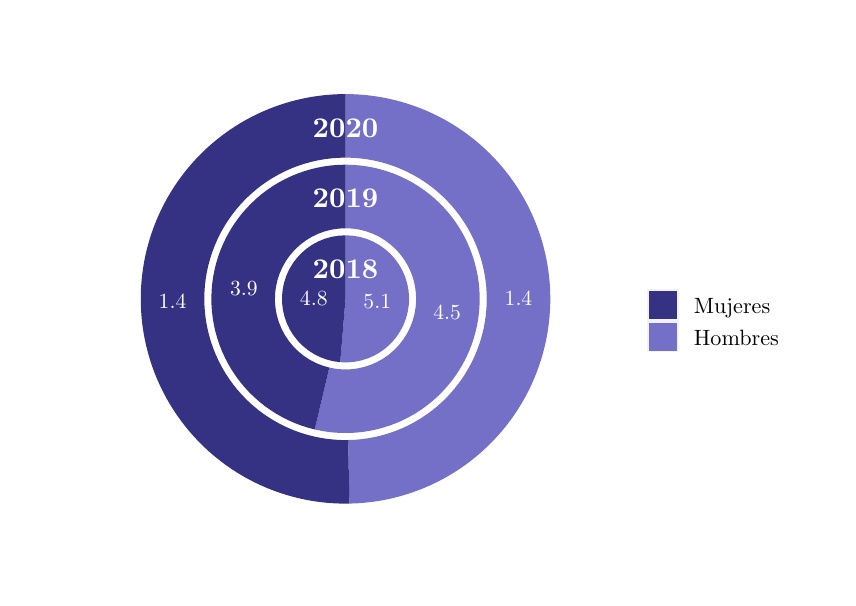
\begin{tikzpicture}[x=1pt,y=1pt]% Created by tikzDevice version 0.12.4 on 2023-05-22 13:40:59
% !TEX encoding = UTF-8 Unicode
\definecolor{fillColor}{RGB}{255,255,255}
\path[use as bounding box,fill=fillColor,fill opacity=0.00] (0,0) rectangle (289.08,198.74);
\begin{scope}
\path[clip] (  0.00,  0.00) rectangle (289.08,198.74);
\definecolor{drawColor}{RGB}{255,255,255}
\definecolor{fillColor}{RGB}{255,255,255}

\path[draw=drawColor,line width= 0.6pt,line join=round,line cap=round,fill=fillColor] ( 14.11,  0.00) rectangle (274.97,198.74);
\end{scope}
\begin{scope}
\path[clip] (  0.00,  0.00) rectangle (289.08,198.74);
\definecolor{fillColor}{RGB}{116,112,200}

\path[fill=fillColor] (114.85,100.75) --
	(114.64, 98.20) --
	(114.43, 95.66) --
	(114.22, 93.12) --
	(114.01, 90.57) --
	(113.80, 88.03) --
	(113.59, 85.49) --
	(113.37, 82.95) --
	(113.16, 80.40) --
	(112.95, 77.86) --
	(115.50, 77.79) --
	(118.05, 78.00) --
	(120.55, 78.50) --
	(122.98, 79.27) --
	(125.32, 80.30) --
	(127.52, 81.59) --
	(129.57, 83.11) --
	(131.43, 84.86) --
	(133.09, 86.79) --
	(134.53, 88.90) --
	(135.72, 91.16) --
	(136.66, 93.54) --
	(137.32, 96.00) --
	(137.71, 98.52) --
	(137.82,101.07) --
	(137.64,103.62) --
	(137.18,106.13) --
	(136.44,108.57) --
	(135.44,110.92) --
	(134.19,113.14) --
	(132.69,115.21) --
	(130.98,117.10) --
	(129.06,118.79) --
	(126.97,120.25) --
	(124.73,121.48) --
	(122.37,122.45) --
	(119.92,123.15) --
	(117.40,123.57) --
	(114.85,123.71) --
	(114.85,121.16) --
	(114.85,118.61) --
	(114.85,116.06) --
	(114.85,113.50) --
	(114.85,110.95) --
	(114.85,108.40) --
	(114.85,105.85) --
	(114.85,103.30) --
	(114.85,100.75) --
	(114.85,100.75) --
	cycle;
\definecolor{fillColor}{RGB}{54,50,131}

\path[fill=fillColor] (114.85,100.75) --
	(114.85,103.30) --
	(114.85,105.85) --
	(114.85,108.40) --
	(114.85,110.95) --
	(114.85,113.50) --
	(114.85,116.06) --
	(114.85,118.61) --
	(114.85,121.16) --
	(114.85,123.71) --
	(112.35,123.57) --
	(109.88,123.16) --
	(107.46,122.49) --
	(105.13,121.55) --
	(102.92,120.37) --
	(100.86,118.95) --
	( 98.95,117.32) --
	( 97.24,115.49) --
	( 95.74,113.48) --
	( 94.47,111.32) --
	( 93.44,109.03) --
	( 92.66,106.65) --
	( 92.15,104.19) --
	( 91.91,101.70) --
	( 91.94, 99.19) --
	( 92.25, 96.70) --
	( 92.82, 94.26) --
	( 93.66, 91.90) --
	( 94.75, 89.64) --
	( 96.08, 87.52) --
	( 97.64, 85.55) --
	( 99.40, 83.76) --
	(101.34, 82.18) --
	(103.45, 80.82) --
	(105.69, 79.69) --
	(108.04, 78.82) --
	(110.47, 78.20) --
	(112.95, 77.86) --
	(113.16, 80.40) --
	(113.37, 82.95) --
	(113.59, 85.49) --
	(113.80, 88.03) --
	(114.01, 90.57) --
	(114.22, 93.12) --
	(114.43, 95.66) --
	(114.64, 98.20) --
	(114.85,100.75) --
	(114.85,100.75) --
	cycle;
\definecolor{fillColor}{RGB}{116,112,200}

\path[fill=fillColor] (109.00, 75.91) --
	(108.42, 73.43) --
	(107.83, 70.94) --
	(107.25, 68.46) --
	(106.66, 65.97) --
	(106.08, 63.49) --
	(105.49, 61.01) --
	(104.91, 58.52) --
	(104.32, 56.04) --
	(103.74, 53.56) --
	(106.20, 53.04) --
	(108.69, 52.66) --
	(111.19, 52.40) --
	(113.70, 52.28) --
	(116.22, 52.28) --
	(118.73, 52.42) --
	(121.23, 52.69) --
	(123.71, 53.08) --
	(126.18, 53.61) --
	(128.60, 54.26) --
	(131.00, 55.03) --
	(133.35, 55.93) --
	(135.65, 56.95) --
	(137.89, 58.09) --
	(140.07, 59.34) --
	(142.19, 60.70) --
	(144.23, 62.18) --
	(146.19, 63.75) --
	(148.06, 65.43) --
	(149.85, 67.20) --
	(151.54, 69.06) --
	(153.14, 71.00) --
	(154.63, 73.03) --
	(156.01, 75.13) --
	(157.29, 77.30) --
	(158.45, 79.53) --
	(159.49, 81.82) --
	(160.41, 84.16) --
	(161.21, 86.55) --
	(161.88, 88.97) --
	(162.43, 91.42) --
	(162.85, 93.90) --
	(163.14, 96.40) --
	(163.30, 98.91) --
	(163.33,101.43) --
	(163.23,103.94) --
	(163.00,106.45) --
	(162.64,108.94) --
	(162.15,111.40) --
	(161.53,113.84) --
	(160.79,116.25) --
	(159.92,118.61) --
	(158.94,120.92) --
	(157.83,123.18) --
	(156.61,125.38) --
	(155.28,127.51) --
	(153.83,129.57) --
	(152.28,131.56) --
	(150.64,133.46) --
	(148.89,135.27) --
	(147.06,136.99) --
	(145.13,138.61) --
	(143.13,140.13) --
	(141.05,141.54) --
	(138.90,142.85) --
	(136.68,144.04) --
	(134.41,145.11) --
	(132.08,146.06) --
	(129.70,146.90) --
	(127.29,147.60) --
	(124.84,148.19) --
	(122.37,148.64) --
	(119.88,148.97) --
	(117.37,149.16) --
	(114.85,149.23) --
	(114.85,146.68) --
	(114.85,144.12) --
	(114.85,141.57) --
	(114.85,139.02) --
	(114.85,136.47) --
	(114.85,133.92) --
	(114.85,131.37) --
	(114.85,128.81) --
	(114.85,126.26) --
	(117.38,126.14) --
	(119.88,125.76) --
	(122.34,125.14) --
	(124.71,124.28) --
	(127.00,123.19) --
	(129.16,121.87) --
	(131.18,120.35) --
	(133.04,118.64) --
	(134.73,116.75) --
	(136.21,114.70) --
	(137.49,112.52) --
	(138.55,110.22) --
	(139.37,107.83) --
	(139.95,105.36) --
	(140.28,102.86) --
	(140.37,100.33) --
	(140.20, 97.80) --
	(139.78, 95.31) --
	(139.12, 92.86) --
	(138.22, 90.50) --
	(137.09, 88.24) --
	(135.74, 86.09) --
	(134.19, 84.10) --
	(132.44, 82.26) --
	(130.53, 80.61) --
	(128.46, 79.16) --
	(126.25, 77.92) --
	(123.94, 76.90) --
	(121.53, 76.12) --
	(119.06, 75.58) --
	(116.54, 75.29) --
	(114.01, 75.24) --
	(111.49, 75.45) --
	(109.00, 75.91) --
	cycle;
\definecolor{fillColor}{RGB}{54,50,131}

\path[fill=fillColor] (114.85,126.26) --
	(114.85,128.81) --
	(114.85,131.37) --
	(114.85,133.92) --
	(114.85,136.47) --
	(114.85,139.02) --
	(114.85,141.57) --
	(114.85,144.12) --
	(114.85,146.68) --
	(114.85,149.23) --
	(112.33,149.16) --
	(109.82,148.97) --
	(107.32,148.64) --
	(104.85,148.18) --
	(102.40,147.60) --
	( 99.98,146.89) --
	( 97.60,146.05) --
	( 95.27,145.10) --
	( 92.99,144.02) --
	( 90.78,142.83) --
	( 88.62,141.52) --
	( 86.54,140.10) --
	( 84.53,138.58) --
	( 82.61,136.95) --
	( 80.77,135.23) --
	( 79.03,133.41) --
	( 77.38,131.51) --
	( 75.83,129.52) --
	( 74.39,127.45) --
	( 73.06,125.31) --
	( 71.84,123.11) --
	( 70.73,120.84) --
	( 69.75,118.53) --
	( 68.89,116.16) --
	( 68.15,113.75) --
	( 67.54,111.31) --
	( 67.05,108.83) --
	( 66.70,106.34) --
	( 66.47,103.83) --
	( 66.38,101.31) --
	( 66.41, 98.80) --
	( 66.58, 96.28) --
	( 66.88, 93.78) --
	( 67.30, 91.30) --
	( 67.86, 88.84) --
	( 68.54, 86.41) --
	( 69.35, 84.03) --
	( 70.28, 81.69) --
	( 71.33, 79.40) --
	( 72.49, 77.16) --
	( 73.78, 75.00) --
	( 75.17, 72.90) --
	( 76.67, 70.87) --
	( 78.27, 68.93) --
	( 79.97, 67.07) --
	( 81.77, 65.31) --
	( 83.66, 63.64) --
	( 85.63, 62.07) --
	( 87.68, 60.60) --
	( 89.80, 59.24) --
	( 91.99, 58.00) --
	( 94.24, 56.87) --
	( 96.55, 55.85) --
	( 98.90, 54.96) --
	(101.30, 54.20) --
	(103.74, 53.56) --
	(104.32, 56.04) --
	(104.91, 58.52) --
	(105.49, 61.01) --
	(106.08, 63.49) --
	(106.66, 65.97) --
	(107.25, 68.46) --
	(107.83, 70.94) --
	(108.42, 73.43) --
	(109.00, 75.91) --
	(106.54, 76.62) --
	(104.17, 77.57) --
	(101.90, 78.76) --
	( 99.76, 80.17) --
	( 97.78, 81.78) --
	( 95.96, 83.59) --
	( 94.34, 85.57) --
	( 92.92, 87.70) --
	( 91.73, 89.96) --
	( 90.76, 92.33) --
	( 90.04, 94.79) --
	( 89.57, 97.31) --
	( 89.35, 99.86) --
	( 89.39,102.42) --
	( 89.69,104.96) --
	( 90.24,107.46) --
	( 91.03,109.89) --
	( 92.07,112.23) --
	( 93.33,114.46) --
	( 94.81,116.54) --
	( 96.50,118.47) --
	( 98.37,120.22) --
	(100.40,121.77) --
	(102.58,123.12) --
	(104.88,124.23) --
	(107.29,125.11) --
	(109.77,125.75) --
	(112.30,126.13) --
	(114.85,126.26) --
	cycle;
\definecolor{fillColor}{RGB}{116,112,200}

\path[fill=fillColor] (115.82, 49.72) --
	(115.86, 47.17) --
	(115.91, 44.62) --
	(115.96, 42.07) --
	(116.01, 39.52) --
	(116.06, 36.97) --
	(116.10, 34.42) --
	(116.15, 31.86) --
	(116.20, 29.31) --
	(116.25, 26.76) --
	(118.76, 26.85) --
	(121.26, 27.03) --
	(123.76, 27.29) --
	(126.25, 27.63) --
	(128.72, 28.06) --
	(131.18, 28.57) --
	(133.62, 29.17) --
	(136.04, 29.85) --
	(138.44, 30.61) --
	(140.80, 31.45) --
	(143.14, 32.37) --
	(145.44, 33.37) --
	(147.71, 34.45) --
	(149.94, 35.60) --
	(152.13, 36.83) --
	(154.28, 38.13) --
	(156.38, 39.50) --
	(158.44, 40.95) --
	(160.44, 42.46) --
	(162.39, 44.04) --
	(164.29, 45.69) --
	(166.13, 47.40) --
	(167.91, 49.17) --
	(169.63, 51.00) --
	(171.29, 52.89) --
	(172.88, 54.83) --
	(174.40, 56.82) --
	(175.86, 58.87) --
	(177.25, 60.97) --
	(178.56, 63.11) --
	(179.80, 65.29) --
	(180.97, 67.51) --
	(182.06, 69.78) --
	(183.07, 72.08) --
	(184.00, 74.41) --
	(184.86, 76.77) --
	(185.63, 79.16) --
	(186.32, 81.57) --
	(186.93, 84.01) --
	(187.46, 86.46) --
	(187.90, 88.94) --
	(188.26, 91.42) --
	(188.53, 93.92) --
	(188.72, 96.42) --
	(188.83, 98.93) --
	(188.85,101.44) --
	(188.78,103.95) --
	(188.63,106.46) --
	(188.39,108.96) --
	(188.07,111.45) --
	(187.67,113.93) --
	(187.18,116.40) --
	(186.60,118.84) --
	(185.95,121.27) --
	(185.21,123.67) --
	(184.39,126.04) --
	(183.49,128.39) --
	(182.52,130.70) --
	(181.46,132.98) --
	(180.33,135.22) --
	(179.12,137.42) --
	(177.84,139.58) --
	(176.49,141.70) --
	(175.06,143.77) --
	(173.57,145.78) --
	(172.00,147.75) --
	(170.38,149.66) --
	(168.68,151.52) --
	(166.93,153.32) --
	(165.12,155.05) --
	(163.24,156.73) --
	(161.32,158.34) --
	(159.33,159.88) --
	(157.30,161.36) --
	(155.22,162.76) --
	(153.09,164.10) --
	(150.92,165.36) --
	(148.71,166.54) --
	(146.46,167.66) --
	(144.17,168.69) --
	(141.84,169.65) --
	(139.49,170.52) --
	(137.11,171.32) --
	(134.70,172.03) --
	(132.27,172.66) --
	(129.82,173.21) --
	(127.35,173.68) --
	(124.87,174.06) --
	(122.37,174.36) --
	(119.87,174.57) --
	(117.36,174.70) --
	(114.85,174.74) --
	(114.85,172.19) --
	(114.85,169.64) --
	(114.85,167.09) --
	(114.85,164.54) --
	(114.85,161.99) --
	(114.85,159.43) --
	(114.85,156.88) --
	(114.85,154.33) --
	(114.85,151.78) --
	(117.38,151.72) --
	(119.90,151.53) --
	(122.41,151.22) --
	(124.90,150.78) --
	(127.37,150.22) --
	(129.81,149.54) --
	(132.21,148.74) --
	(134.56,147.82) --
	(136.87,146.78) --
	(139.12,145.64) --
	(141.32,144.38) --
	(143.45,143.01) --
	(145.51,141.55) --
	(147.49,139.98) --
	(149.40,138.31) --
	(151.21,136.55) --
	(152.94,134.71) --
	(154.58,132.78) --
	(156.12,130.77) --
	(157.55,128.69) --
	(158.89,126.54) --
	(160.11,124.33) --
	(161.22,122.06) --
	(162.22,119.73) --
	(163.10,117.36) --
	(163.87,114.95) --
	(164.51,112.50) --
	(165.03,110.03) --
	(165.43,107.53) --
	(165.71,105.02) --
	(165.86,102.49) --
	(165.88, 99.96) --
	(165.78, 97.44) --
	(165.55, 94.92) --
	(165.20, 92.41) --
	(164.73, 89.93) --
	(164.13, 87.47) --
	(163.41, 85.04) --
	(162.57, 82.66) --
	(161.62, 80.32) --
	(160.55, 78.02) --
	(159.37, 75.79) --
	(158.07, 73.61) --
	(156.68, 71.50) --
	(155.18, 69.47) --
	(153.58, 67.51) --
	(151.88, 65.63) --
	(150.10, 63.84) --
	(148.23, 62.14) --
	(146.27, 60.53) --
	(144.24, 59.03) --
	(142.14, 57.62) --
	(139.97, 56.32) --
	(137.74, 55.13) --
	(135.45, 54.05) --
	(133.11, 53.09) --
	(130.73, 52.24) --
	(128.30, 51.52) --
	(125.85, 50.91) --
	(123.36, 50.43) --
	(120.86, 50.07) --
	(118.34, 49.83) --
	(115.82, 49.72) --
	cycle;
\definecolor{fillColor}{RGB}{54,50,131}

\path[fill=fillColor] (114.85,151.78) --
	(114.85,154.33) --
	(114.85,156.88) --
	(114.85,159.43) --
	(114.85,161.99) --
	(114.85,164.54) --
	(114.85,167.09) --
	(114.85,169.64) --
	(114.85,172.19) --
	(114.85,174.74) --
	(112.34,174.70) --
	(109.83,174.57) --
	(107.32,174.36) --
	(104.83,174.06) --
	(102.34,173.68) --
	( 99.87,173.21) --
	( 97.42,172.66) --
	( 94.98,172.03) --
	( 92.57,171.31) --
	( 90.19,170.51) --
	( 87.83,169.63) --
	( 85.51,168.68) --
	( 83.22,167.64) --
	( 80.96,166.53) --
	( 78.75,165.34) --
	( 76.57,164.07) --
	( 74.44,162.73) --
	( 72.36,161.33) --
	( 70.33,159.85) --
	( 68.34,158.30) --
	( 66.41,156.69) --
	( 64.54,155.01) --
	( 62.73,153.27) --
	( 60.97,151.47) --
	( 59.28,149.61) --
	( 57.65,147.69) --
	( 56.09,145.72) --
	( 54.60,143.70) --
	( 53.17,141.62) --
	( 51.82,139.51) --
	( 50.54,137.34) --
	( 49.33,135.13) --
	( 48.20,132.89) --
	( 47.15,130.61) --
	( 46.17,128.29) --
	( 45.28,125.94) --
	( 44.46,123.56) --
	( 43.73,121.15) --
	( 43.07,118.73) --
	( 42.50,116.28) --
	( 42.02,113.81) --
	( 41.62,111.33) --
	( 41.30,108.83) --
	( 41.07,106.33) --
	( 40.92,103.82) --
	( 40.86,101.31) --
	( 40.88, 98.79) --
	( 40.99, 96.28) --
	( 41.19, 93.77) --
	( 41.46, 91.27) --
	( 41.83, 88.78) --
	( 42.28, 86.31) --
	( 42.81, 83.85) --
	( 43.43, 81.42) --
	( 44.12, 79.00) --
	( 44.90, 76.61) --
	( 45.76, 74.25) --
	( 46.70, 71.91) --
	( 47.72, 69.62) --
	( 48.82, 67.35) --
	( 49.99, 65.13) --
	( 51.24, 62.94) --
	( 52.56, 60.81) --
	( 53.95, 58.71) --
	( 55.42, 56.67) --
	( 56.95, 54.67) --
	( 58.55, 52.73) --
	( 60.21, 50.85) --
	( 61.94, 49.02) --
	( 63.73, 47.25) --
	( 65.57, 45.54) --
	( 67.48, 43.90) --
	( 69.44, 42.33) --
	( 71.45, 40.82) --
	( 73.51, 39.38) --
	( 75.62, 38.01) --
	( 77.77, 36.71) --
	( 79.97, 35.49) --
	( 82.21, 34.34) --
	( 84.48, 33.27) --
	( 86.79, 32.28) --
	( 89.14, 31.36) --
	( 91.51, 30.53) --
	( 93.91, 29.78) --
	( 96.33, 29.10) --
	( 98.78, 28.52) --
	(101.24, 28.01) --
	(103.72, 27.59) --
	(106.21, 27.26) --
	(108.71, 27.00) --
	(111.22, 26.84) --
	(113.73, 26.76) --
	(116.25, 26.76) --
	(116.20, 29.31) --
	(116.15, 31.86) --
	(116.10, 34.42) --
	(116.06, 36.97) --
	(116.01, 39.52) --
	(115.96, 42.07) --
	(115.91, 44.62) --
	(115.86, 47.17) --
	(115.82, 49.72) --
	(113.30, 49.74) --
	(110.78, 49.88) --
	(108.27, 50.14) --
	(105.78, 50.53) --
	(103.32, 51.04) --
	(100.88, 51.67) --
	( 98.47, 52.41) --
	( 96.10, 53.28) --
	( 93.78, 54.27) --
	( 91.52, 55.36) --
	( 89.30, 56.57) --
	( 87.15, 57.88) --
	( 85.07, 59.30) --
	( 83.06, 60.82) --
	( 81.13, 62.44) --
	( 79.28, 64.15) --
	( 77.52, 65.95) --
	( 75.85, 67.84) --
	( 74.27, 69.81) --
	( 72.79, 71.85) --
	( 71.42, 73.96) --
	( 70.15, 76.13) --
	( 68.99, 78.37) --
	( 67.94, 80.66) --
	( 67.00, 83.00) --
	( 66.19, 85.39) --
	( 65.49, 87.81) --
	( 64.91, 90.26) --
	( 64.45, 92.74) --
	( 64.12, 95.24) --
	( 63.91, 97.75) --
	( 63.82,100.26) --
	( 63.86,102.78) --
	( 64.02,105.30) --
	( 64.31,107.80) --
	( 64.72,110.29) --
	( 65.25,112.75) --
	( 65.91,115.19) --
	( 66.68,117.58) --
	( 67.57,119.94) --
	( 68.57,122.25) --
	( 69.69,124.51) --
	( 70.92,126.71) --
	( 72.25,128.85) --
	( 73.69,130.92) --
	( 75.23,132.91) --
	( 76.87,134.83) --
	( 78.60,136.66) --
	( 80.41,138.41) --
	( 82.32,140.06) --
	( 84.30,141.62) --
	( 86.35,143.08) --
	( 88.48,144.43) --
	( 90.66,145.68) --
	( 92.91,146.82) --
	( 95.21,147.85) --
	( 97.56,148.76) --
	( 99.95,149.55) --
	(102.38,150.23) --
	(104.84,150.79) --
	(107.32,151.22) --
	(109.82,151.53) --
	(112.33,151.72) --
	(114.85,151.78) --
	cycle;
\definecolor{drawColor}{RGB}{255,255,255}

\node[text=drawColor,anchor=base,inner sep=0pt, outer sep=0pt, scale=  0.78] at (126.33, 97.24) {5.1};

\node[text=drawColor,anchor=base,inner sep=0pt, outer sep=0pt, scale=  0.78] at (103.38, 98.19) {4.8};

\node[text=drawColor,anchor=base,inner sep=0pt, outer sep=0pt, scale=  0.78] at (151.60, 93.44) {4.5};

\node[text=drawColor,anchor=base,inner sep=0pt, outer sep=0pt, scale=  0.78] at ( 78.10,101.98) {3.9};

\node[text=drawColor,anchor=base,inner sep=0pt, outer sep=0pt, scale=  0.78] at (177.36, 98.30) {1.4};

\node[text=drawColor,anchor=base,inner sep=0pt, outer sep=0pt, scale=  0.78] at ( 52.34, 97.12) {1.4};

\node[text=drawColor,anchor=base,inner sep=0pt, outer sep=0pt, scale=  1.03] at (114.85,108.18) {\bfseries 2018};

\node[text=drawColor,anchor=base,inner sep=0pt, outer sep=0pt, scale=  1.03] at (114.85,133.70) {\bfseries 2019};

\node[text=drawColor,anchor=base,inner sep=0pt, outer sep=0pt, scale=  1.03] at (114.85,159.22) {\bfseries 2020};
\end{scope}
\begin{scope}
\path[clip] (  0.00,  0.00) rectangle (289.08,198.74);
\definecolor{fillColor}{RGB}{255,255,255}

\path[fill=fillColor] (218.35, 75.89) rectangle (269.47,125.60);
\end{scope}
\begin{scope}
\path[clip] (  0.00,  0.00) rectangle (289.08,198.74);
\definecolor{fillColor}{gray}{0.95}

\path[fill=fillColor] (223.85, 92.77) rectangle (235.23,104.15);
\end{scope}
\begin{scope}
\path[clip] (  0.00,  0.00) rectangle (289.08,198.74);
\definecolor{fillColor}{RGB}{54,50,131}

\path[fill=fillColor] (224.51, 93.44) rectangle (234.57,103.49);
\end{scope}
\begin{scope}
\path[clip] (  0.00,  0.00) rectangle (289.08,198.74);
\definecolor{fillColor}{gray}{0.95}

\path[fill=fillColor] (223.85, 81.39) rectangle (235.23, 92.77);
\end{scope}
\begin{scope}
\path[clip] (  0.00,  0.00) rectangle (289.08,198.74);
\definecolor{fillColor}{RGB}{116,112,200}

\path[fill=fillColor] (224.51, 82.05) rectangle (234.57, 92.11);
\end{scope}
\begin{scope}
\path[clip] (  0.00,  0.00) rectangle (289.08,198.74);
\definecolor{drawColor}{RGB}{0,0,0}

\node[text=drawColor,anchor=base west,inner sep=0pt, outer sep=0pt, scale=  0.80] at (240.73, 95.34) {Mujeres};
\end{scope}
\begin{scope}
\path[clip] (  0.00,  0.00) rectangle (289.08,198.74);
\definecolor{drawColor}{RGB}{0,0,0}

\node[text=drawColor,anchor=base west,inner sep=0pt, outer sep=0pt, scale=  0.80] at (240.73, 83.96) {Hombres};
\end{scope}
\end{tikzpicture}}{Estadísticas de Educación INE, con datos proporcionados por el Ministerio de Educación}{}

\cajita{REVISAR Tasa de deserción en el nivel básico por sexo}{En Guatemala, de 2018 a 2020 los hombres presentaron una mayor tasa de deserción en el ciclo básico que las mujeres. La deserción escolar de mujeres disminuyó de 2018 a 2020 en 2.3.}{Tasa de deserción en el nivel básico por sexo (porcentaje)}{República de Guatemala, Instituto Nacional de Estadística}{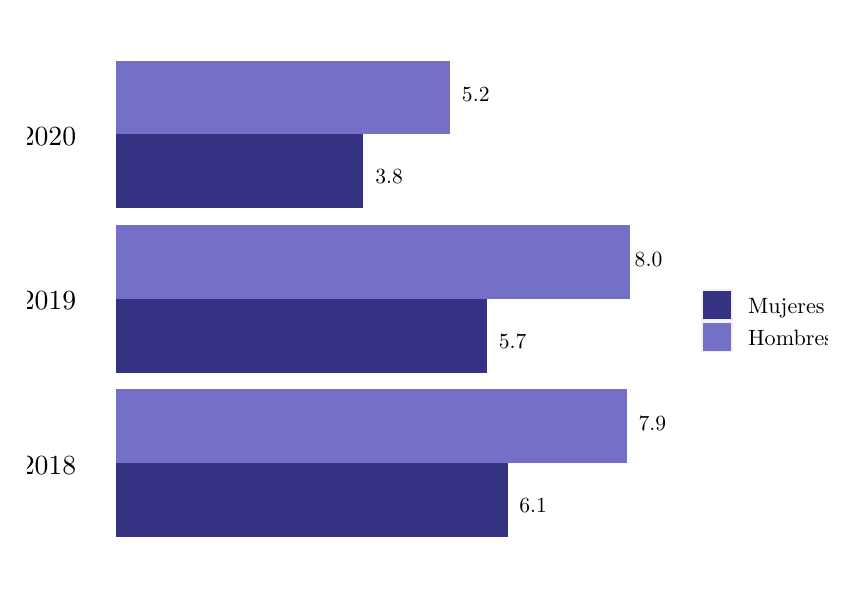
\begin{tikzpicture}[x=1pt,y=1pt]% Created by tikzDevice version 0.12.4 on 2023-05-29 13:43:34
% !TEX encoding = UTF-8 Unicode
\definecolor{fillColor}{RGB}{255,255,255}
\path[use as bounding box,fill=fillColor,fill opacity=0.00] (0,0) rectangle (289.08,198.74);
\begin{scope}
\path[clip] (  0.00,  0.00) rectangle (289.08,198.74);

\path[] (  0.00,  0.00) rectangle (289.08,198.74);
\end{scope}
\begin{scope}
\path[clip] (  0.00,  0.00) rectangle (289.08,198.74);
\definecolor{fillColor}{RGB}{54,50,131}

\path[fill=fillColor] ( 31.76, 14.63) rectangle (173.40, 41.35);
\definecolor{fillColor}{RGB}{116,112,200}

\path[fill=fillColor] ( 31.76, 41.35) rectangle (216.47, 68.08);
\definecolor{fillColor}{RGB}{54,50,131}

\path[fill=fillColor] ( 31.76, 74.02) rectangle (165.97,100.75);
\definecolor{fillColor}{RGB}{116,112,200}

\path[fill=fillColor] ( 31.76,100.75) rectangle (217.66,127.47);
\definecolor{fillColor}{RGB}{54,50,131}

\path[fill=fillColor] ( 31.76,133.41) rectangle (121.33,160.14);
\definecolor{fillColor}{RGB}{116,112,200}

\path[fill=fillColor] ( 31.76,160.14) rectangle (152.65,186.86);
\definecolor{drawColor}{RGB}{0,0,0}

\node[text=drawColor,anchor=base west,inner sep=0pt, outer sep=0pt, scale=  0.78] at (177.67, 23.47) {6.1};

\node[text=drawColor,anchor=base west,inner sep=0pt, outer sep=0pt, scale=  0.78] at (220.75, 53.17) {7.9};

\node[text=drawColor,anchor=base west,inner sep=0pt, outer sep=0pt, scale=  0.78] at (170.24, 82.87) {5.7};

\node[text=drawColor,anchor=base west,inner sep=0pt, outer sep=0pt, scale=  0.78] at (219.36,112.56) {8.0};

\node[text=drawColor,anchor=base west,inner sep=0pt, outer sep=0pt, scale=  0.78] at (125.61,142.26) {3.8};

\node[text=drawColor,anchor=base west,inner sep=0pt, outer sep=0pt, scale=  0.78] at (156.93,171.95) {5.2};

\path[] ( 22.47, 41.35) --
	(226.96, 41.35);

\path[] ( 22.47,100.75) --
	(226.96,100.75);

\path[] ( 22.47,160.14) --
	(226.96,160.14);

\path[] ( 22.47,  2.75) rectangle (226.96,198.74);
\end{scope}
\begin{scope}
\path[clip] (  0.00,  0.00) rectangle (289.08,198.74);

\path[] ( 22.47,  2.75) --
	( 22.47,198.74);
\end{scope}
\begin{scope}
\path[clip] (  0.00,  0.00) rectangle (289.08,198.74);
\definecolor{drawColor}{RGB}{0,0,0}

\node[text=drawColor,anchor=base east,inner sep=0pt, outer sep=0pt, scale=  1.00] at ( 17.52, 37.45) {2018};

\node[text=drawColor,anchor=base east,inner sep=0pt, outer sep=0pt, scale=  1.00] at ( 17.52, 96.84) {2019};

\node[text=drawColor,anchor=base east,inner sep=0pt, outer sep=0pt, scale=  1.00] at ( 17.52,156.23) {2020};
\end{scope}
\begin{scope}
\path[clip] (  0.00,  0.00) rectangle (289.08,198.74);

\path[] ( 19.72, 41.35) --
	( 22.47, 41.35);

\path[] ( 19.72,100.75) --
	( 22.47,100.75);

\path[] ( 19.72,160.14) --
	( 22.47,160.14);
\end{scope}
\begin{scope}
\path[clip] (  0.00,  0.00) rectangle (289.08,198.74);

\path[] ( 22.47,  2.75) --
	(226.96,  2.75);
\end{scope}
\begin{scope}
\path[clip] (  0.00,  0.00) rectangle (289.08,198.74);

\path[] ( 31.76,  0.00) --
	( 31.76,  2.75);

\path[] ( 78.45,  0.00) --
	( 78.45,  2.75);

\path[] (125.14,  0.00) --
	(125.14,  2.75);

\path[] (171.83,  0.00) --
	(171.83,  2.75);

\path[] (218.51,  0.00) --
	(218.51,  2.75);
\end{scope}
\begin{scope}
\path[clip] (  0.00,  0.00) rectangle (289.08,198.74);
\definecolor{fillColor}{RGB}{255,255,255}

\path[fill=fillColor] (237.96, 75.89) rectangle (289.08,125.60);
\end{scope}
\begin{scope}
\path[clip] (  0.00,  0.00) rectangle (289.08,198.74);
\definecolor{fillColor}{gray}{0.95}

\path[fill=fillColor] (243.46, 92.77) rectangle (254.84,104.15);
\end{scope}
\begin{scope}
\path[clip] (  0.00,  0.00) rectangle (289.08,198.74);
\definecolor{fillColor}{RGB}{54,50,131}

\path[fill=fillColor] (244.12, 93.44) rectangle (254.17,103.49);
\end{scope}
\begin{scope}
\path[clip] (  0.00,  0.00) rectangle (289.08,198.74);
\definecolor{fillColor}{gray}{0.95}

\path[fill=fillColor] (243.46, 81.39) rectangle (254.84, 92.77);
\end{scope}
\begin{scope}
\path[clip] (  0.00,  0.00) rectangle (289.08,198.74);
\definecolor{fillColor}{RGB}{116,112,200}

\path[fill=fillColor] (244.12, 82.05) rectangle (254.17, 92.11);
\end{scope}
\begin{scope}
\path[clip] (  0.00,  0.00) rectangle (289.08,198.74);
\definecolor{drawColor}{RGB}{0,0,0}

\node[text=drawColor,anchor=base west,inner sep=0pt, outer sep=0pt, scale=  0.80] at (260.34, 95.34) {Mujeres};
\end{scope}
\begin{scope}
\path[clip] (  0.00,  0.00) rectangle (289.08,198.74);
\definecolor{drawColor}{RGB}{0,0,0}

\node[text=drawColor,anchor=base west,inner sep=0pt, outer sep=0pt, scale=  0.80] at (260.34, 83.96) {Hombres};
\end{scope}
\end{tikzpicture}}{Estadísticas de Educación INE, con datos proporcionados por el Ministerio de Educación}{}

\cajota{REVISAR Tasa de deserción en el nivel primario por sexo, según departamento}{En Guatemala se obsevó una disminución de en la tasa de deserción en el nivel primario de 2019 a 2020. La mayor tasa de deserción de mujeres en primaria fue reportada en Petén en 2018, con una tasa de 12.0. Sololá reportó la menor tasa para mujeres en 2020. }{Tasa de deserción en el nivel primario por sexo, según departamento (porcentaje)}{República de Guatemala, Instituto Nacional de Estadística}{\begin{tabular}[t]{ccccccc}
\toprule
\multicolumn{1}{c}{\textbf{ }} & \multicolumn{2}{c}{\textbf{2018}} & \multicolumn{2}{c}{\textbf{2019}} & \multicolumn{2}{c}{\textbf{2020}} \\
\cmidrule(l{3pt}r{3pt}){2-3} \cmidrule(l{3pt}r{3pt}){4-5} \cmidrule(l{3pt}r{3pt}){6-7}
\textbf{Departamento} & \textbf{Mujeres} & \textbf{Hombres} & \textbf{Mujeres} & \textbf{Hombres} & \textbf{Mujeres} & \textbf{Hombres}\\
\midrule
\cellcolor[HTML]{B6B3FF}{Guatemala} & \cellcolor[HTML]{B6B3FF}{3.1} & \cellcolor[HTML]{B6B3FF}{3.8} & \cellcolor[HTML]{B6B3FF}{2.5} & \cellcolor[HTML]{B6B3FF}{3.3} & \cellcolor[HTML]{B6B3FF}{0.9} & \cellcolor[HTML]{B6B3FF}{1.1}\\
El Progreso & 5.7 & 6.9 & 4.0 & 5.2 & 0.8 & 1.1\\
\cellcolor[HTML]{B6B3FF}{Sacatepéquez} & \cellcolor[HTML]{B6B3FF}{3.4} & \cellcolor[HTML]{B6B3FF}{4.1} & \cellcolor[HTML]{B6B3FF}{2.4} & \cellcolor[HTML]{B6B3FF}{3.0} & \cellcolor[HTML]{B6B3FF}{1.1} & \cellcolor[HTML]{B6B3FF}{1.6}\\
Chimaltenango & 4.2 & 4.5 & 2.5 & 3.0 & 1.6 & 1.5\\
\cellcolor[HTML]{B6B3FF}{Escuintla} & \cellcolor[HTML]{B6B3FF}{7.9} & \cellcolor[HTML]{B6B3FF}{9.1} & \cellcolor[HTML]{B6B3FF}{5.9} & \cellcolor[HTML]{B6B3FF}{7.1} & \cellcolor[HTML]{B6B3FF}{1.5} & \cellcolor[HTML]{B6B3FF}{1.5}\\
Santa Rosa & 4.3 & 5.4 & 4.1 & 5.2 & 1.3 & 1.5\\
\cellcolor[HTML]{B6B3FF}{Sololá} & \cellcolor[HTML]{B6B3FF}{2.7} & \cellcolor[HTML]{B6B3FF}{3.2} & \cellcolor[HTML]{B6B3FF}{1.8} & \cellcolor[HTML]{B6B3FF}{2.1} & \cellcolor[HTML]{B6B3FF}{0.6} & \cellcolor[HTML]{B6B3FF}{0.9}\\
Totonicapán & 5.0 & 5.2 & 2.8 & 3.4 & 1.5 & 1.5\\
\cellcolor[HTML]{B6B3FF}{Quetzaltenango} & \cellcolor[HTML]{B6B3FF}{4.0} & \cellcolor[HTML]{B6B3FF}{4.6} & \cellcolor[HTML]{B6B3FF}{2.8} & \cellcolor[HTML]{B6B3FF}{3.4} & \cellcolor[HTML]{B6B3FF}{1.2} & \cellcolor[HTML]{B6B3FF}{1.3}\\
Suchitepéquez & 7.3 & 7.3 & 5.8 & 6.1 & 1.9 & 1.7\\
\cellcolor[HTML]{B6B3FF}{Retalhuleu} & \cellcolor[HTML]{B6B3FF}{6.0} & \cellcolor[HTML]{B6B3FF}{6.4} & \cellcolor[HTML]{B6B3FF}{4.1} & \cellcolor[HTML]{B6B3FF}{4.9} & \cellcolor[HTML]{B6B3FF}{1.6} & \cellcolor[HTML]{B6B3FF}{1.7}\\
San Marcos & 4.9 & 5.5 & 4.2 & 5.1 & 1.2 & 1.3\\
\cellcolor[HTML]{B6B3FF}{Huehuetenango} & \cellcolor[HTML]{B6B3FF}{8.8} & \cellcolor[HTML]{B6B3FF}{9.4} & \cellcolor[HTML]{B6B3FF}{6.5} & \cellcolor[HTML]{B6B3FF}{7.8} & \cellcolor[HTML]{B6B3FF}{2.4} & \cellcolor[HTML]{B6B3FF}{2.3}\\
Quiché & 6.4 & 6.4 & 4.6 & 5.5 & 2.1 & 1.9\\
\cellcolor[HTML]{B6B3FF}{Baja Verapaz} & \cellcolor[HTML]{B6B3FF}{5.3} & \cellcolor[HTML]{B6B3FF}{5.6} & \cellcolor[HTML]{B6B3FF}{5.3} & \cellcolor[HTML]{B6B3FF}{5.9} & \cellcolor[HTML]{B6B3FF}{1.8} & \cellcolor[HTML]{B6B3FF}{1.7}\\
Alta Verapaz & 6.1 & 5.0 & 4.1 & 4.1 & 2.3 & 1.7\\
\cellcolor[HTML]{B6B3FF}{Petén} & \cellcolor[HTML]{B6B3FF}{12.0} & \cellcolor[HTML]{B6B3FF}{13.2} & \cellcolor[HTML]{B6B3FF}{11.1} & \cellcolor[HTML]{B6B3FF}{12.8} & \cellcolor[HTML]{B6B3FF}{3.2} & \cellcolor[HTML]{B6B3FF}{3.5}\\
Izabal & 7.3 & 8.4 & 6.3 & 7.7 & 1.7 & 1.8\\
\cellcolor[HTML]{B6B3FF}{Zacapa} & \cellcolor[HTML]{B6B3FF}{8.0} & \cellcolor[HTML]{B6B3FF}{9.7} & \cellcolor[HTML]{B6B3FF}{5.3} & \cellcolor[HTML]{B6B3FF}{6.7} & \cellcolor[HTML]{B6B3FF}{2.1} & \cellcolor[HTML]{B6B3FF}{2.5}\\
Chiquimula & 6.2 & 7.1 & 6.1 & 8.0 & 1.7 & 1.9\\
\cellcolor[HTML]{B6B3FF}{Jalapa} & \cellcolor[HTML]{B6B3FF}{7.1} & \cellcolor[HTML]{B6B3FF}{7.8} & \cellcolor[HTML]{B6B3FF}{7.1} & \cellcolor[HTML]{B6B3FF}{8.0} & \cellcolor[HTML]{B6B3FF}{1.7} & \cellcolor[HTML]{B6B3FF}{1.6}\\
Jutiapa & 4.4 & 5.3 & 4.7 & 6.1 & 1.4 & 1.6\\
\bottomrule
\end{tabular}
}{Estadísticas de Educación INE, con datos proporcionados por el Ministerio de Educación}

\cajota{REVISAR Tasa de deserción en el nivel básico por sexo, según departamento}{En Guatemala se observó una disminución en la tasa de deserción en el ciclo básico de 2018 a 2020. La mayor tasa de deserción de mujeres en ciclo básico fue reportada en Petén en 2018, con una tasa de 21.0. Las tasas de deserción de mujeres en Guatemala y en Baja Verapaz son considerablemente menores que las de los hombres de 2018 a 2020.}{Tasa de deserción en el nivel básico por sexo, según departamento (porcentaje)}{República de Guatemala, Instituto Nacional de Estadística}{\begin{tabular}[t]{ccccccc}
\toprule
\multicolumn{1}{c}{\textbf{ }} & \multicolumn{2}{c}{\textbf{2018}} & \multicolumn{2}{c}{\textbf{2019}} & \multicolumn{2}{c}{\textbf{2020}} \\
\cmidrule(l{3pt}r{3pt}){2-3} \cmidrule(l{3pt}r{3pt}){4-5} \cmidrule(l{3pt}r{3pt}){6-7}
\textbf{Departamento} & \textbf{Mujeres} & \textbf{Hombres} & \textbf{Mujeres} & \textbf{Hombres} & \textbf{Mujeres} & \textbf{Hombres}\\
\midrule
\cellcolor[HTML]{B6B3FF}{Guatemala} & \cellcolor[HTML]{B6B3FF}{8.6} & \cellcolor[HTML]{B6B3FF}{13.4} & \cellcolor[HTML]{B6B3FF}{7.9} & \cellcolor[HTML]{B6B3FF}{12.9} & \cellcolor[HTML]{B6B3FF}{5.9} & \cellcolor[HTML]{B6B3FF}{9.4}\\
El Progreso & 9.8 & 14.0 & 9.2 & 12.6 & 4.7 & 7.0\\
\cellcolor[HTML]{B6B3FF}{Sacatepéquez} & \cellcolor[HTML]{B6B3FF}{7.8} & \cellcolor[HTML]{B6B3FF}{12.1} & \cellcolor[HTML]{B6B3FF}{6.4} & \cellcolor[HTML]{B6B3FF}{10.9} & \cellcolor[HTML]{B6B3FF}{3.4} & \cellcolor[HTML]{B6B3FF}{6.8}\\
Chimaltenango & 0.8 & 10.6 & 5.8 & 9.3 & 5.7 & 8.7\\
\cellcolor[HTML]{B6B3FF}{Escuintla} & \cellcolor[HTML]{B6B3FF}{9.3} & \cellcolor[HTML]{B6B3FF}{12.2} & \cellcolor[HTML]{B6B3FF}{8.3} & \cellcolor[HTML]{B6B3FF}{11.1} & \cellcolor[HTML]{B6B3FF}{3.3} & \cellcolor[HTML]{B6B3FF}{4.6}\\
Santa Rosa & 6.3 & 8.6 & 7.5 & 10.9 & 5.0 & 5.6\\
\cellcolor[HTML]{B6B3FF}{Sololá} & \cellcolor[HTML]{B6B3FF}{5.8} & \cellcolor[HTML]{B6B3FF}{9.0} & \cellcolor[HTML]{B6B3FF}{4.1} & \cellcolor[HTML]{B6B3FF}{7.7} & \cellcolor[HTML]{B6B3FF}{4.7} & \cellcolor[HTML]{B6B3FF}{6.6}\\
Totonicapán & 7.1 & 9.5 & 5.8 & 9.2 & 4.4 & 5.5\\
\cellcolor[HTML]{B6B3FF}{Quetzaltenango} & \cellcolor[HTML]{B6B3FF}{6.3} & \cellcolor[HTML]{B6B3FF}{9.2} & \cellcolor[HTML]{B6B3FF}{5.4} & \cellcolor[HTML]{B6B3FF}{7.6} & \cellcolor[HTML]{B6B3FF}{3.4} & \cellcolor[HTML]{B6B3FF}{4.7}\\
Suchitepéquez & 8.2 & 11.4 & 6.9 & 11.3 & 2.6 & 3.5\\
\cellcolor[HTML]{B6B3FF}{Retalhuleu} & \cellcolor[HTML]{B6B3FF}{7.5} & \cellcolor[HTML]{B6B3FF}{9.8} & \cellcolor[HTML]{B6B3FF}{7.0} & \cellcolor[HTML]{B6B3FF}{9.3} & \cellcolor[HTML]{B6B3FF}{5.3} & \cellcolor[HTML]{B6B3FF}{6.9}\\
San Marcos & 7.6 & 9.8 & 7.4 & 9.6 & 4.9 & 6.5\\
\cellcolor[HTML]{B6B3FF}{Huehuetenango} & \cellcolor[HTML]{B6B3FF}{12.5} & \cellcolor[HTML]{B6B3FF}{17.5} & \cellcolor[HTML]{B6B3FF}{11.2} & \cellcolor[HTML]{B6B3FF}{16.6} & \cellcolor[HTML]{B6B3FF}{6.8} & \cellcolor[HTML]{B6B3FF}{9.9}\\
El Quiche & 8.5 & 12.8 & 7.4 & 12.4 & 4.8 & 6.6\\
\cellcolor[HTML]{B6B3FF}{Baja Verapaz} & \cellcolor[HTML]{B6B3FF}{9.7} & \cellcolor[HTML]{B6B3FF}{13.7} & \cellcolor[HTML]{B6B3FF}{10.1} & \cellcolor[HTML]{B6B3FF}{18.6} & \cellcolor[HTML]{B6B3FF}{5.2} & \cellcolor[HTML]{B6B3FF}{9.3}\\
Alta Verapaz & 7.3 & 7.4 & 6.9 & 8.3 & 4.7 & 4.9\\
\cellcolor[HTML]{B6B3FF}{Petén} & \cellcolor[HTML]{B6B3FF}{21.0} & \cellcolor[HTML]{B6B3FF}{28.9} & \cellcolor[HTML]{B6B3FF}{20.1} & \cellcolor[HTML]{B6B3FF}{28.1} & \cellcolor[HTML]{B6B3FF}{12.5} & \cellcolor[HTML]{B6B3FF}{16.8}\\
Izabal & 12.5 & 17.1 & 12.6 & 19.0 & 9.8 & 13.4\\
\cellcolor[HTML]{B6B3FF}{Zacapa} & \cellcolor[HTML]{B6B3FF}{11.8} & \cellcolor[HTML]{B6B3FF}{15.6} & \cellcolor[HTML]{B6B3FF}{9.2} & \cellcolor[HTML]{B6B3FF}{14.3} & \cellcolor[HTML]{B6B3FF}{6.0} & \cellcolor[HTML]{B6B3FF}{8.5}\\
Chiquimula & 13.2 & 18.3 & 12.2 & 17.3 & 7.3 & 10.1\\
\cellcolor[HTML]{B6B3FF}{Jalapa} & \cellcolor[HTML]{B6B3FF}{11.4} & \cellcolor[HTML]{B6B3FF}{14.4} & \cellcolor[HTML]{B6B3FF}{12.1} & \cellcolor[HTML]{B6B3FF}{17.9} & \cellcolor[HTML]{B6B3FF}{5.5} & \cellcolor[HTML]{B6B3FF}{8.4}\\
Jutiapa & 8.5 & 11.8 & 9.7 & 14.0 & 4.7 & 6.7\\
\bottomrule
\end{tabular}
}{Estadísticas de Educación INE, con datos proporcionados por el Ministerio de Educación}

\cajita{REVISAR Tasa de deserción en el nivel primario por sexo}{La tasa neta de deserción es la relación porcentual entre el total de deserción en el ciclo escolar y la población matriculada en dicho ciclo.

La gráfica muestra que en 2018 y 2019 los hombres reportaron tasas de deserción en el nivel primario mayores que las mujeres. En el 2020 se reportaron iguales tasas para hombres y mujeres de 1.4 respectivamente. }{Tasa de deserción en el nivel primario por sexo (porcentaje)}{República de Guatemala, Instituto Nacional de Estadística}{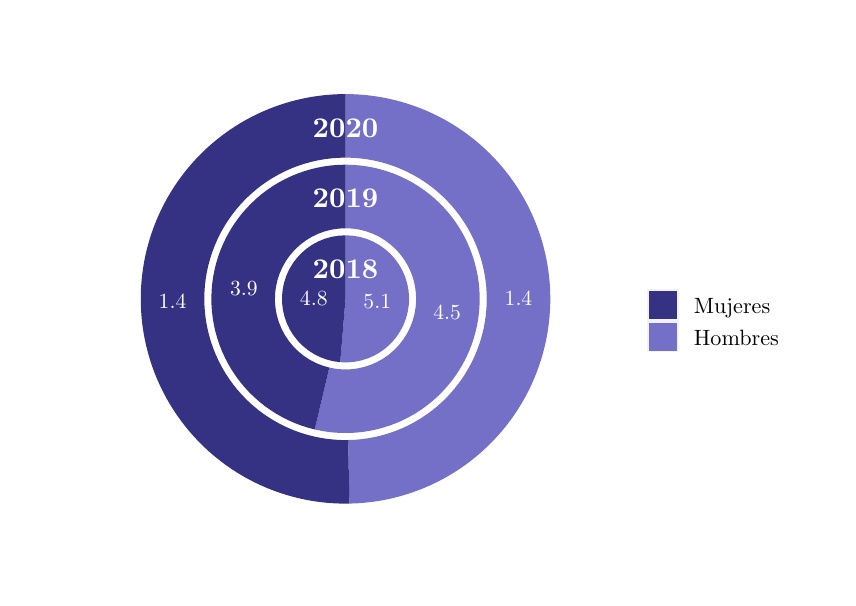
\begin{tikzpicture}[x=1pt,y=1pt]% Created by tikzDevice version 0.12.4 on 2023-05-22 13:40:59
% !TEX encoding = UTF-8 Unicode
\definecolor{fillColor}{RGB}{255,255,255}
\path[use as bounding box,fill=fillColor,fill opacity=0.00] (0,0) rectangle (289.08,198.74);
\begin{scope}
\path[clip] (  0.00,  0.00) rectangle (289.08,198.74);
\definecolor{drawColor}{RGB}{255,255,255}
\definecolor{fillColor}{RGB}{255,255,255}

\path[draw=drawColor,line width= 0.6pt,line join=round,line cap=round,fill=fillColor] ( 14.11,  0.00) rectangle (274.97,198.74);
\end{scope}
\begin{scope}
\path[clip] (  0.00,  0.00) rectangle (289.08,198.74);
\definecolor{fillColor}{RGB}{116,112,200}

\path[fill=fillColor] (114.85,100.75) --
	(114.64, 98.20) --
	(114.43, 95.66) --
	(114.22, 93.12) --
	(114.01, 90.57) --
	(113.80, 88.03) --
	(113.59, 85.49) --
	(113.37, 82.95) --
	(113.16, 80.40) --
	(112.95, 77.86) --
	(115.50, 77.79) --
	(118.05, 78.00) --
	(120.55, 78.50) --
	(122.98, 79.27) --
	(125.32, 80.30) --
	(127.52, 81.59) --
	(129.57, 83.11) --
	(131.43, 84.86) --
	(133.09, 86.79) --
	(134.53, 88.90) --
	(135.72, 91.16) --
	(136.66, 93.54) --
	(137.32, 96.00) --
	(137.71, 98.52) --
	(137.82,101.07) --
	(137.64,103.62) --
	(137.18,106.13) --
	(136.44,108.57) --
	(135.44,110.92) --
	(134.19,113.14) --
	(132.69,115.21) --
	(130.98,117.10) --
	(129.06,118.79) --
	(126.97,120.25) --
	(124.73,121.48) --
	(122.37,122.45) --
	(119.92,123.15) --
	(117.40,123.57) --
	(114.85,123.71) --
	(114.85,121.16) --
	(114.85,118.61) --
	(114.85,116.06) --
	(114.85,113.50) --
	(114.85,110.95) --
	(114.85,108.40) --
	(114.85,105.85) --
	(114.85,103.30) --
	(114.85,100.75) --
	(114.85,100.75) --
	cycle;
\definecolor{fillColor}{RGB}{54,50,131}

\path[fill=fillColor] (114.85,100.75) --
	(114.85,103.30) --
	(114.85,105.85) --
	(114.85,108.40) --
	(114.85,110.95) --
	(114.85,113.50) --
	(114.85,116.06) --
	(114.85,118.61) --
	(114.85,121.16) --
	(114.85,123.71) --
	(112.35,123.57) --
	(109.88,123.16) --
	(107.46,122.49) --
	(105.13,121.55) --
	(102.92,120.37) --
	(100.86,118.95) --
	( 98.95,117.32) --
	( 97.24,115.49) --
	( 95.74,113.48) --
	( 94.47,111.32) --
	( 93.44,109.03) --
	( 92.66,106.65) --
	( 92.15,104.19) --
	( 91.91,101.70) --
	( 91.94, 99.19) --
	( 92.25, 96.70) --
	( 92.82, 94.26) --
	( 93.66, 91.90) --
	( 94.75, 89.64) --
	( 96.08, 87.52) --
	( 97.64, 85.55) --
	( 99.40, 83.76) --
	(101.34, 82.18) --
	(103.45, 80.82) --
	(105.69, 79.69) --
	(108.04, 78.82) --
	(110.47, 78.20) --
	(112.95, 77.86) --
	(113.16, 80.40) --
	(113.37, 82.95) --
	(113.59, 85.49) --
	(113.80, 88.03) --
	(114.01, 90.57) --
	(114.22, 93.12) --
	(114.43, 95.66) --
	(114.64, 98.20) --
	(114.85,100.75) --
	(114.85,100.75) --
	cycle;
\definecolor{fillColor}{RGB}{116,112,200}

\path[fill=fillColor] (109.00, 75.91) --
	(108.42, 73.43) --
	(107.83, 70.94) --
	(107.25, 68.46) --
	(106.66, 65.97) --
	(106.08, 63.49) --
	(105.49, 61.01) --
	(104.91, 58.52) --
	(104.32, 56.04) --
	(103.74, 53.56) --
	(106.20, 53.04) --
	(108.69, 52.66) --
	(111.19, 52.40) --
	(113.70, 52.28) --
	(116.22, 52.28) --
	(118.73, 52.42) --
	(121.23, 52.69) --
	(123.71, 53.08) --
	(126.18, 53.61) --
	(128.60, 54.26) --
	(131.00, 55.03) --
	(133.35, 55.93) --
	(135.65, 56.95) --
	(137.89, 58.09) --
	(140.07, 59.34) --
	(142.19, 60.70) --
	(144.23, 62.18) --
	(146.19, 63.75) --
	(148.06, 65.43) --
	(149.85, 67.20) --
	(151.54, 69.06) --
	(153.14, 71.00) --
	(154.63, 73.03) --
	(156.01, 75.13) --
	(157.29, 77.30) --
	(158.45, 79.53) --
	(159.49, 81.82) --
	(160.41, 84.16) --
	(161.21, 86.55) --
	(161.88, 88.97) --
	(162.43, 91.42) --
	(162.85, 93.90) --
	(163.14, 96.40) --
	(163.30, 98.91) --
	(163.33,101.43) --
	(163.23,103.94) --
	(163.00,106.45) --
	(162.64,108.94) --
	(162.15,111.40) --
	(161.53,113.84) --
	(160.79,116.25) --
	(159.92,118.61) --
	(158.94,120.92) --
	(157.83,123.18) --
	(156.61,125.38) --
	(155.28,127.51) --
	(153.83,129.57) --
	(152.28,131.56) --
	(150.64,133.46) --
	(148.89,135.27) --
	(147.06,136.99) --
	(145.13,138.61) --
	(143.13,140.13) --
	(141.05,141.54) --
	(138.90,142.85) --
	(136.68,144.04) --
	(134.41,145.11) --
	(132.08,146.06) --
	(129.70,146.90) --
	(127.29,147.60) --
	(124.84,148.19) --
	(122.37,148.64) --
	(119.88,148.97) --
	(117.37,149.16) --
	(114.85,149.23) --
	(114.85,146.68) --
	(114.85,144.12) --
	(114.85,141.57) --
	(114.85,139.02) --
	(114.85,136.47) --
	(114.85,133.92) --
	(114.85,131.37) --
	(114.85,128.81) --
	(114.85,126.26) --
	(117.38,126.14) --
	(119.88,125.76) --
	(122.34,125.14) --
	(124.71,124.28) --
	(127.00,123.19) --
	(129.16,121.87) --
	(131.18,120.35) --
	(133.04,118.64) --
	(134.73,116.75) --
	(136.21,114.70) --
	(137.49,112.52) --
	(138.55,110.22) --
	(139.37,107.83) --
	(139.95,105.36) --
	(140.28,102.86) --
	(140.37,100.33) --
	(140.20, 97.80) --
	(139.78, 95.31) --
	(139.12, 92.86) --
	(138.22, 90.50) --
	(137.09, 88.24) --
	(135.74, 86.09) --
	(134.19, 84.10) --
	(132.44, 82.26) --
	(130.53, 80.61) --
	(128.46, 79.16) --
	(126.25, 77.92) --
	(123.94, 76.90) --
	(121.53, 76.12) --
	(119.06, 75.58) --
	(116.54, 75.29) --
	(114.01, 75.24) --
	(111.49, 75.45) --
	(109.00, 75.91) --
	cycle;
\definecolor{fillColor}{RGB}{54,50,131}

\path[fill=fillColor] (114.85,126.26) --
	(114.85,128.81) --
	(114.85,131.37) --
	(114.85,133.92) --
	(114.85,136.47) --
	(114.85,139.02) --
	(114.85,141.57) --
	(114.85,144.12) --
	(114.85,146.68) --
	(114.85,149.23) --
	(112.33,149.16) --
	(109.82,148.97) --
	(107.32,148.64) --
	(104.85,148.18) --
	(102.40,147.60) --
	( 99.98,146.89) --
	( 97.60,146.05) --
	( 95.27,145.10) --
	( 92.99,144.02) --
	( 90.78,142.83) --
	( 88.62,141.52) --
	( 86.54,140.10) --
	( 84.53,138.58) --
	( 82.61,136.95) --
	( 80.77,135.23) --
	( 79.03,133.41) --
	( 77.38,131.51) --
	( 75.83,129.52) --
	( 74.39,127.45) --
	( 73.06,125.31) --
	( 71.84,123.11) --
	( 70.73,120.84) --
	( 69.75,118.53) --
	( 68.89,116.16) --
	( 68.15,113.75) --
	( 67.54,111.31) --
	( 67.05,108.83) --
	( 66.70,106.34) --
	( 66.47,103.83) --
	( 66.38,101.31) --
	( 66.41, 98.80) --
	( 66.58, 96.28) --
	( 66.88, 93.78) --
	( 67.30, 91.30) --
	( 67.86, 88.84) --
	( 68.54, 86.41) --
	( 69.35, 84.03) --
	( 70.28, 81.69) --
	( 71.33, 79.40) --
	( 72.49, 77.16) --
	( 73.78, 75.00) --
	( 75.17, 72.90) --
	( 76.67, 70.87) --
	( 78.27, 68.93) --
	( 79.97, 67.07) --
	( 81.77, 65.31) --
	( 83.66, 63.64) --
	( 85.63, 62.07) --
	( 87.68, 60.60) --
	( 89.80, 59.24) --
	( 91.99, 58.00) --
	( 94.24, 56.87) --
	( 96.55, 55.85) --
	( 98.90, 54.96) --
	(101.30, 54.20) --
	(103.74, 53.56) --
	(104.32, 56.04) --
	(104.91, 58.52) --
	(105.49, 61.01) --
	(106.08, 63.49) --
	(106.66, 65.97) --
	(107.25, 68.46) --
	(107.83, 70.94) --
	(108.42, 73.43) --
	(109.00, 75.91) --
	(106.54, 76.62) --
	(104.17, 77.57) --
	(101.90, 78.76) --
	( 99.76, 80.17) --
	( 97.78, 81.78) --
	( 95.96, 83.59) --
	( 94.34, 85.57) --
	( 92.92, 87.70) --
	( 91.73, 89.96) --
	( 90.76, 92.33) --
	( 90.04, 94.79) --
	( 89.57, 97.31) --
	( 89.35, 99.86) --
	( 89.39,102.42) --
	( 89.69,104.96) --
	( 90.24,107.46) --
	( 91.03,109.89) --
	( 92.07,112.23) --
	( 93.33,114.46) --
	( 94.81,116.54) --
	( 96.50,118.47) --
	( 98.37,120.22) --
	(100.40,121.77) --
	(102.58,123.12) --
	(104.88,124.23) --
	(107.29,125.11) --
	(109.77,125.75) --
	(112.30,126.13) --
	(114.85,126.26) --
	cycle;
\definecolor{fillColor}{RGB}{116,112,200}

\path[fill=fillColor] (115.82, 49.72) --
	(115.86, 47.17) --
	(115.91, 44.62) --
	(115.96, 42.07) --
	(116.01, 39.52) --
	(116.06, 36.97) --
	(116.10, 34.42) --
	(116.15, 31.86) --
	(116.20, 29.31) --
	(116.25, 26.76) --
	(118.76, 26.85) --
	(121.26, 27.03) --
	(123.76, 27.29) --
	(126.25, 27.63) --
	(128.72, 28.06) --
	(131.18, 28.57) --
	(133.62, 29.17) --
	(136.04, 29.85) --
	(138.44, 30.61) --
	(140.80, 31.45) --
	(143.14, 32.37) --
	(145.44, 33.37) --
	(147.71, 34.45) --
	(149.94, 35.60) --
	(152.13, 36.83) --
	(154.28, 38.13) --
	(156.38, 39.50) --
	(158.44, 40.95) --
	(160.44, 42.46) --
	(162.39, 44.04) --
	(164.29, 45.69) --
	(166.13, 47.40) --
	(167.91, 49.17) --
	(169.63, 51.00) --
	(171.29, 52.89) --
	(172.88, 54.83) --
	(174.40, 56.82) --
	(175.86, 58.87) --
	(177.25, 60.97) --
	(178.56, 63.11) --
	(179.80, 65.29) --
	(180.97, 67.51) --
	(182.06, 69.78) --
	(183.07, 72.08) --
	(184.00, 74.41) --
	(184.86, 76.77) --
	(185.63, 79.16) --
	(186.32, 81.57) --
	(186.93, 84.01) --
	(187.46, 86.46) --
	(187.90, 88.94) --
	(188.26, 91.42) --
	(188.53, 93.92) --
	(188.72, 96.42) --
	(188.83, 98.93) --
	(188.85,101.44) --
	(188.78,103.95) --
	(188.63,106.46) --
	(188.39,108.96) --
	(188.07,111.45) --
	(187.67,113.93) --
	(187.18,116.40) --
	(186.60,118.84) --
	(185.95,121.27) --
	(185.21,123.67) --
	(184.39,126.04) --
	(183.49,128.39) --
	(182.52,130.70) --
	(181.46,132.98) --
	(180.33,135.22) --
	(179.12,137.42) --
	(177.84,139.58) --
	(176.49,141.70) --
	(175.06,143.77) --
	(173.57,145.78) --
	(172.00,147.75) --
	(170.38,149.66) --
	(168.68,151.52) --
	(166.93,153.32) --
	(165.12,155.05) --
	(163.24,156.73) --
	(161.32,158.34) --
	(159.33,159.88) --
	(157.30,161.36) --
	(155.22,162.76) --
	(153.09,164.10) --
	(150.92,165.36) --
	(148.71,166.54) --
	(146.46,167.66) --
	(144.17,168.69) --
	(141.84,169.65) --
	(139.49,170.52) --
	(137.11,171.32) --
	(134.70,172.03) --
	(132.27,172.66) --
	(129.82,173.21) --
	(127.35,173.68) --
	(124.87,174.06) --
	(122.37,174.36) --
	(119.87,174.57) --
	(117.36,174.70) --
	(114.85,174.74) --
	(114.85,172.19) --
	(114.85,169.64) --
	(114.85,167.09) --
	(114.85,164.54) --
	(114.85,161.99) --
	(114.85,159.43) --
	(114.85,156.88) --
	(114.85,154.33) --
	(114.85,151.78) --
	(117.38,151.72) --
	(119.90,151.53) --
	(122.41,151.22) --
	(124.90,150.78) --
	(127.37,150.22) --
	(129.81,149.54) --
	(132.21,148.74) --
	(134.56,147.82) --
	(136.87,146.78) --
	(139.12,145.64) --
	(141.32,144.38) --
	(143.45,143.01) --
	(145.51,141.55) --
	(147.49,139.98) --
	(149.40,138.31) --
	(151.21,136.55) --
	(152.94,134.71) --
	(154.58,132.78) --
	(156.12,130.77) --
	(157.55,128.69) --
	(158.89,126.54) --
	(160.11,124.33) --
	(161.22,122.06) --
	(162.22,119.73) --
	(163.10,117.36) --
	(163.87,114.95) --
	(164.51,112.50) --
	(165.03,110.03) --
	(165.43,107.53) --
	(165.71,105.02) --
	(165.86,102.49) --
	(165.88, 99.96) --
	(165.78, 97.44) --
	(165.55, 94.92) --
	(165.20, 92.41) --
	(164.73, 89.93) --
	(164.13, 87.47) --
	(163.41, 85.04) --
	(162.57, 82.66) --
	(161.62, 80.32) --
	(160.55, 78.02) --
	(159.37, 75.79) --
	(158.07, 73.61) --
	(156.68, 71.50) --
	(155.18, 69.47) --
	(153.58, 67.51) --
	(151.88, 65.63) --
	(150.10, 63.84) --
	(148.23, 62.14) --
	(146.27, 60.53) --
	(144.24, 59.03) --
	(142.14, 57.62) --
	(139.97, 56.32) --
	(137.74, 55.13) --
	(135.45, 54.05) --
	(133.11, 53.09) --
	(130.73, 52.24) --
	(128.30, 51.52) --
	(125.85, 50.91) --
	(123.36, 50.43) --
	(120.86, 50.07) --
	(118.34, 49.83) --
	(115.82, 49.72) --
	cycle;
\definecolor{fillColor}{RGB}{54,50,131}

\path[fill=fillColor] (114.85,151.78) --
	(114.85,154.33) --
	(114.85,156.88) --
	(114.85,159.43) --
	(114.85,161.99) --
	(114.85,164.54) --
	(114.85,167.09) --
	(114.85,169.64) --
	(114.85,172.19) --
	(114.85,174.74) --
	(112.34,174.70) --
	(109.83,174.57) --
	(107.32,174.36) --
	(104.83,174.06) --
	(102.34,173.68) --
	( 99.87,173.21) --
	( 97.42,172.66) --
	( 94.98,172.03) --
	( 92.57,171.31) --
	( 90.19,170.51) --
	( 87.83,169.63) --
	( 85.51,168.68) --
	( 83.22,167.64) --
	( 80.96,166.53) --
	( 78.75,165.34) --
	( 76.57,164.07) --
	( 74.44,162.73) --
	( 72.36,161.33) --
	( 70.33,159.85) --
	( 68.34,158.30) --
	( 66.41,156.69) --
	( 64.54,155.01) --
	( 62.73,153.27) --
	( 60.97,151.47) --
	( 59.28,149.61) --
	( 57.65,147.69) --
	( 56.09,145.72) --
	( 54.60,143.70) --
	( 53.17,141.62) --
	( 51.82,139.51) --
	( 50.54,137.34) --
	( 49.33,135.13) --
	( 48.20,132.89) --
	( 47.15,130.61) --
	( 46.17,128.29) --
	( 45.28,125.94) --
	( 44.46,123.56) --
	( 43.73,121.15) --
	( 43.07,118.73) --
	( 42.50,116.28) --
	( 42.02,113.81) --
	( 41.62,111.33) --
	( 41.30,108.83) --
	( 41.07,106.33) --
	( 40.92,103.82) --
	( 40.86,101.31) --
	( 40.88, 98.79) --
	( 40.99, 96.28) --
	( 41.19, 93.77) --
	( 41.46, 91.27) --
	( 41.83, 88.78) --
	( 42.28, 86.31) --
	( 42.81, 83.85) --
	( 43.43, 81.42) --
	( 44.12, 79.00) --
	( 44.90, 76.61) --
	( 45.76, 74.25) --
	( 46.70, 71.91) --
	( 47.72, 69.62) --
	( 48.82, 67.35) --
	( 49.99, 65.13) --
	( 51.24, 62.94) --
	( 52.56, 60.81) --
	( 53.95, 58.71) --
	( 55.42, 56.67) --
	( 56.95, 54.67) --
	( 58.55, 52.73) --
	( 60.21, 50.85) --
	( 61.94, 49.02) --
	( 63.73, 47.25) --
	( 65.57, 45.54) --
	( 67.48, 43.90) --
	( 69.44, 42.33) --
	( 71.45, 40.82) --
	( 73.51, 39.38) --
	( 75.62, 38.01) --
	( 77.77, 36.71) --
	( 79.97, 35.49) --
	( 82.21, 34.34) --
	( 84.48, 33.27) --
	( 86.79, 32.28) --
	( 89.14, 31.36) --
	( 91.51, 30.53) --
	( 93.91, 29.78) --
	( 96.33, 29.10) --
	( 98.78, 28.52) --
	(101.24, 28.01) --
	(103.72, 27.59) --
	(106.21, 27.26) --
	(108.71, 27.00) --
	(111.22, 26.84) --
	(113.73, 26.76) --
	(116.25, 26.76) --
	(116.20, 29.31) --
	(116.15, 31.86) --
	(116.10, 34.42) --
	(116.06, 36.97) --
	(116.01, 39.52) --
	(115.96, 42.07) --
	(115.91, 44.62) --
	(115.86, 47.17) --
	(115.82, 49.72) --
	(113.30, 49.74) --
	(110.78, 49.88) --
	(108.27, 50.14) --
	(105.78, 50.53) --
	(103.32, 51.04) --
	(100.88, 51.67) --
	( 98.47, 52.41) --
	( 96.10, 53.28) --
	( 93.78, 54.27) --
	( 91.52, 55.36) --
	( 89.30, 56.57) --
	( 87.15, 57.88) --
	( 85.07, 59.30) --
	( 83.06, 60.82) --
	( 81.13, 62.44) --
	( 79.28, 64.15) --
	( 77.52, 65.95) --
	( 75.85, 67.84) --
	( 74.27, 69.81) --
	( 72.79, 71.85) --
	( 71.42, 73.96) --
	( 70.15, 76.13) --
	( 68.99, 78.37) --
	( 67.94, 80.66) --
	( 67.00, 83.00) --
	( 66.19, 85.39) --
	( 65.49, 87.81) --
	( 64.91, 90.26) --
	( 64.45, 92.74) --
	( 64.12, 95.24) --
	( 63.91, 97.75) --
	( 63.82,100.26) --
	( 63.86,102.78) --
	( 64.02,105.30) --
	( 64.31,107.80) --
	( 64.72,110.29) --
	( 65.25,112.75) --
	( 65.91,115.19) --
	( 66.68,117.58) --
	( 67.57,119.94) --
	( 68.57,122.25) --
	( 69.69,124.51) --
	( 70.92,126.71) --
	( 72.25,128.85) --
	( 73.69,130.92) --
	( 75.23,132.91) --
	( 76.87,134.83) --
	( 78.60,136.66) --
	( 80.41,138.41) --
	( 82.32,140.06) --
	( 84.30,141.62) --
	( 86.35,143.08) --
	( 88.48,144.43) --
	( 90.66,145.68) --
	( 92.91,146.82) --
	( 95.21,147.85) --
	( 97.56,148.76) --
	( 99.95,149.55) --
	(102.38,150.23) --
	(104.84,150.79) --
	(107.32,151.22) --
	(109.82,151.53) --
	(112.33,151.72) --
	(114.85,151.78) --
	cycle;
\definecolor{drawColor}{RGB}{255,255,255}

\node[text=drawColor,anchor=base,inner sep=0pt, outer sep=0pt, scale=  0.78] at (126.33, 97.24) {5.1};

\node[text=drawColor,anchor=base,inner sep=0pt, outer sep=0pt, scale=  0.78] at (103.38, 98.19) {4.8};

\node[text=drawColor,anchor=base,inner sep=0pt, outer sep=0pt, scale=  0.78] at (151.60, 93.44) {4.5};

\node[text=drawColor,anchor=base,inner sep=0pt, outer sep=0pt, scale=  0.78] at ( 78.10,101.98) {3.9};

\node[text=drawColor,anchor=base,inner sep=0pt, outer sep=0pt, scale=  0.78] at (177.36, 98.30) {1.4};

\node[text=drawColor,anchor=base,inner sep=0pt, outer sep=0pt, scale=  0.78] at ( 52.34, 97.12) {1.4};

\node[text=drawColor,anchor=base,inner sep=0pt, outer sep=0pt, scale=  1.03] at (114.85,108.18) {\bfseries 2018};

\node[text=drawColor,anchor=base,inner sep=0pt, outer sep=0pt, scale=  1.03] at (114.85,133.70) {\bfseries 2019};

\node[text=drawColor,anchor=base,inner sep=0pt, outer sep=0pt, scale=  1.03] at (114.85,159.22) {\bfseries 2020};
\end{scope}
\begin{scope}
\path[clip] (  0.00,  0.00) rectangle (289.08,198.74);
\definecolor{fillColor}{RGB}{255,255,255}

\path[fill=fillColor] (218.35, 75.89) rectangle (269.47,125.60);
\end{scope}
\begin{scope}
\path[clip] (  0.00,  0.00) rectangle (289.08,198.74);
\definecolor{fillColor}{gray}{0.95}

\path[fill=fillColor] (223.85, 92.77) rectangle (235.23,104.15);
\end{scope}
\begin{scope}
\path[clip] (  0.00,  0.00) rectangle (289.08,198.74);
\definecolor{fillColor}{RGB}{54,50,131}

\path[fill=fillColor] (224.51, 93.44) rectangle (234.57,103.49);
\end{scope}
\begin{scope}
\path[clip] (  0.00,  0.00) rectangle (289.08,198.74);
\definecolor{fillColor}{gray}{0.95}

\path[fill=fillColor] (223.85, 81.39) rectangle (235.23, 92.77);
\end{scope}
\begin{scope}
\path[clip] (  0.00,  0.00) rectangle (289.08,198.74);
\definecolor{fillColor}{RGB}{116,112,200}

\path[fill=fillColor] (224.51, 82.05) rectangle (234.57, 92.11);
\end{scope}
\begin{scope}
\path[clip] (  0.00,  0.00) rectangle (289.08,198.74);
\definecolor{drawColor}{RGB}{0,0,0}

\node[text=drawColor,anchor=base west,inner sep=0pt, outer sep=0pt, scale=  0.80] at (240.73, 95.34) {Mujeres};
\end{scope}
\begin{scope}
\path[clip] (  0.00,  0.00) rectangle (289.08,198.74);
\definecolor{drawColor}{RGB}{0,0,0}

\node[text=drawColor,anchor=base west,inner sep=0pt, outer sep=0pt, scale=  0.80] at (240.73, 83.96) {Hombres};
\end{scope}
\end{tikzpicture}}{Estadísticas de Educación INE, con datos proporcionados por el Ministerio de Educación}{}

\cajita{REVISAR Tasa de deserción en el nivel básico por sexo}{En Guatemala, de 2018 a 2020 los hombres presentaron una mayor tasa de deserción en el ciclo básico que las mujeres. La deserción escolar de mujeres disminuyó de 2018 a 2020 en 2.3.}{Tasa de deserción en el nivel básico por sexo (porcentaje)}{República de Guatemala, Instituto Nacional de Estadística}{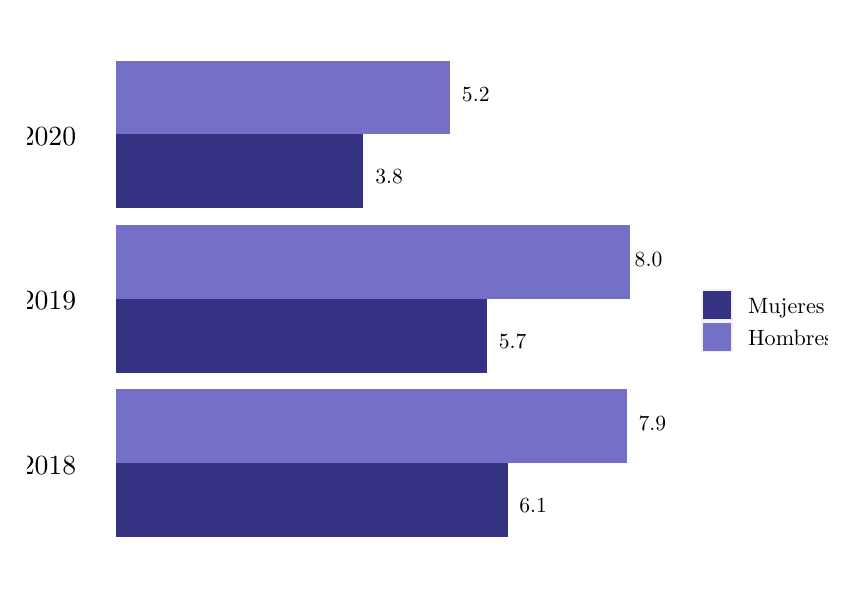
\begin{tikzpicture}[x=1pt,y=1pt]% Created by tikzDevice version 0.12.4 on 2023-05-29 13:43:34
% !TEX encoding = UTF-8 Unicode
\definecolor{fillColor}{RGB}{255,255,255}
\path[use as bounding box,fill=fillColor,fill opacity=0.00] (0,0) rectangle (289.08,198.74);
\begin{scope}
\path[clip] (  0.00,  0.00) rectangle (289.08,198.74);

\path[] (  0.00,  0.00) rectangle (289.08,198.74);
\end{scope}
\begin{scope}
\path[clip] (  0.00,  0.00) rectangle (289.08,198.74);
\definecolor{fillColor}{RGB}{54,50,131}

\path[fill=fillColor] ( 31.76, 14.63) rectangle (173.40, 41.35);
\definecolor{fillColor}{RGB}{116,112,200}

\path[fill=fillColor] ( 31.76, 41.35) rectangle (216.47, 68.08);
\definecolor{fillColor}{RGB}{54,50,131}

\path[fill=fillColor] ( 31.76, 74.02) rectangle (165.97,100.75);
\definecolor{fillColor}{RGB}{116,112,200}

\path[fill=fillColor] ( 31.76,100.75) rectangle (217.66,127.47);
\definecolor{fillColor}{RGB}{54,50,131}

\path[fill=fillColor] ( 31.76,133.41) rectangle (121.33,160.14);
\definecolor{fillColor}{RGB}{116,112,200}

\path[fill=fillColor] ( 31.76,160.14) rectangle (152.65,186.86);
\definecolor{drawColor}{RGB}{0,0,0}

\node[text=drawColor,anchor=base west,inner sep=0pt, outer sep=0pt, scale=  0.78] at (177.67, 23.47) {6.1};

\node[text=drawColor,anchor=base west,inner sep=0pt, outer sep=0pt, scale=  0.78] at (220.75, 53.17) {7.9};

\node[text=drawColor,anchor=base west,inner sep=0pt, outer sep=0pt, scale=  0.78] at (170.24, 82.87) {5.7};

\node[text=drawColor,anchor=base west,inner sep=0pt, outer sep=0pt, scale=  0.78] at (219.36,112.56) {8.0};

\node[text=drawColor,anchor=base west,inner sep=0pt, outer sep=0pt, scale=  0.78] at (125.61,142.26) {3.8};

\node[text=drawColor,anchor=base west,inner sep=0pt, outer sep=0pt, scale=  0.78] at (156.93,171.95) {5.2};

\path[] ( 22.47, 41.35) --
	(226.96, 41.35);

\path[] ( 22.47,100.75) --
	(226.96,100.75);

\path[] ( 22.47,160.14) --
	(226.96,160.14);

\path[] ( 22.47,  2.75) rectangle (226.96,198.74);
\end{scope}
\begin{scope}
\path[clip] (  0.00,  0.00) rectangle (289.08,198.74);

\path[] ( 22.47,  2.75) --
	( 22.47,198.74);
\end{scope}
\begin{scope}
\path[clip] (  0.00,  0.00) rectangle (289.08,198.74);
\definecolor{drawColor}{RGB}{0,0,0}

\node[text=drawColor,anchor=base east,inner sep=0pt, outer sep=0pt, scale=  1.00] at ( 17.52, 37.45) {2018};

\node[text=drawColor,anchor=base east,inner sep=0pt, outer sep=0pt, scale=  1.00] at ( 17.52, 96.84) {2019};

\node[text=drawColor,anchor=base east,inner sep=0pt, outer sep=0pt, scale=  1.00] at ( 17.52,156.23) {2020};
\end{scope}
\begin{scope}
\path[clip] (  0.00,  0.00) rectangle (289.08,198.74);

\path[] ( 19.72, 41.35) --
	( 22.47, 41.35);

\path[] ( 19.72,100.75) --
	( 22.47,100.75);

\path[] ( 19.72,160.14) --
	( 22.47,160.14);
\end{scope}
\begin{scope}
\path[clip] (  0.00,  0.00) rectangle (289.08,198.74);

\path[] ( 22.47,  2.75) --
	(226.96,  2.75);
\end{scope}
\begin{scope}
\path[clip] (  0.00,  0.00) rectangle (289.08,198.74);

\path[] ( 31.76,  0.00) --
	( 31.76,  2.75);

\path[] ( 78.45,  0.00) --
	( 78.45,  2.75);

\path[] (125.14,  0.00) --
	(125.14,  2.75);

\path[] (171.83,  0.00) --
	(171.83,  2.75);

\path[] (218.51,  0.00) --
	(218.51,  2.75);
\end{scope}
\begin{scope}
\path[clip] (  0.00,  0.00) rectangle (289.08,198.74);
\definecolor{fillColor}{RGB}{255,255,255}

\path[fill=fillColor] (237.96, 75.89) rectangle (289.08,125.60);
\end{scope}
\begin{scope}
\path[clip] (  0.00,  0.00) rectangle (289.08,198.74);
\definecolor{fillColor}{gray}{0.95}

\path[fill=fillColor] (243.46, 92.77) rectangle (254.84,104.15);
\end{scope}
\begin{scope}
\path[clip] (  0.00,  0.00) rectangle (289.08,198.74);
\definecolor{fillColor}{RGB}{54,50,131}

\path[fill=fillColor] (244.12, 93.44) rectangle (254.17,103.49);
\end{scope}
\begin{scope}
\path[clip] (  0.00,  0.00) rectangle (289.08,198.74);
\definecolor{fillColor}{gray}{0.95}

\path[fill=fillColor] (243.46, 81.39) rectangle (254.84, 92.77);
\end{scope}
\begin{scope}
\path[clip] (  0.00,  0.00) rectangle (289.08,198.74);
\definecolor{fillColor}{RGB}{116,112,200}

\path[fill=fillColor] (244.12, 82.05) rectangle (254.17, 92.11);
\end{scope}
\begin{scope}
\path[clip] (  0.00,  0.00) rectangle (289.08,198.74);
\definecolor{drawColor}{RGB}{0,0,0}

\node[text=drawColor,anchor=base west,inner sep=0pt, outer sep=0pt, scale=  0.80] at (260.34, 95.34) {Mujeres};
\end{scope}
\begin{scope}
\path[clip] (  0.00,  0.00) rectangle (289.08,198.74);
\definecolor{drawColor}{RGB}{0,0,0}

\node[text=drawColor,anchor=base west,inner sep=0pt, outer sep=0pt, scale=  0.80] at (260.34, 83.96) {Hombres};
\end{scope}
\end{tikzpicture}}{Estadísticas de Educación INE, con datos proporcionados por el Ministerio de Educación}{}